\documentclass[a4paper,12pt]{article}
\usepackage[lmargin=30mm,rmargin=30mm,tmargin=25mm,bmargin=25mm]{geometry}
\usepackage[utf8]{inputenc}
\usepackage[T1]{fontenc}
\usepackage{newtxtext} 

\usepackage{textcomp}
\usepackage{fdsymbol}
\usepackage{stmaryrd}
\usepackage{underscore}


\usepackage{newunicodechar}
\newunicodechar{Γ}{$\Gamma$}
\newunicodechar{ε}{$\epsilon$}
\newunicodechar{λ}{$\lambda$}
\newunicodechar{ρ}{$\rho$}
\newunicodechar{σ}{$\sigma$}
\newunicodechar{τ}{$\tau$}
\newunicodechar{∷}{$\Colon$} % requires fdsymbol
%\newunicodechar{∷}{$::$}
\newunicodechar{●}{$\smblkcircle$}
%\newunicodechar{→}{$\rightarrow$} % not needed
\newunicodechar{⇒}{$\Rightarrow$}
\newunicodechar{⟹}{$\Longrightarrow$} % unused
%\newunicodechar{⊹}{$\hermitmatrix$} % requires stix
%\newunicodechar{⊹}{$+$}
\newunicodechar{⊹}{$\Diamond$}
\newunicodechar{⟦}{$\llbracket$}
\newunicodechar{⟧}{$\rrbracket$}
\newunicodechar{⟪}{$\langle\!\langle$}
\newunicodechar{⟫}{$\rangle\!\rangle$}
\newunicodechar{⟨}{$\langle$}
\newunicodechar{⟩}{$\rangle$}
%\newunicodechar{·}{$\cdot$} % not needed
\newunicodechar{⊔}{$\sqcup$}
\newunicodechar{⊓}{$\sqcap$}
\newunicodechar{∈}{$\in$}
%\newunicodechar{¬}{$\neg$} % not needed
\newunicodechar{≡}{$\equiv$}
\newunicodechar{≢}{$\neq$}
\newunicodechar{≤}{$\leq$}
\newunicodechar{≰}{$\nleq$}
\newunicodechar{⊑}{$\sqsubseteq$}
\newunicodechar{ℕ}{$\mathbb{N}$}
\newunicodechar{∘}{$\circ$}
\newunicodechar{₁}{\textsubscript{1}}
\newunicodechar{₂}{\textsubscript{2}}
\newunicodechar{₃}{\textsubscript{3}}
\newunicodechar{η}{$\eta$}
\newunicodechar{⊤}{$\top$}

\usepackage[estonian]{babel}
%\usepackage[none]{hyphenat}


\usepackage{fancyhdr}
\fancypagestyle{FirstPage}{\fancyhf{}\renewcommand{\headrulewidth}{0pt}\fancyfoot[C]{Tallinn 2017}}

\addto\captionsestonian{
  \renewcommand*\contentsname{\centering Sisukord}
  \renewcommand*\listfigurename{\centering Jooniste loetelu}
  \renewcommand*\refname{Kasutatud kirjandus}
}

\usepackage{hyperref}

\usepackage[figure,table]{totalcount}

%\linespread{1.4}
%\renewcommand{\baselinestretch}{1.5}

\setlength{\parindent}{0pt}
\setlength{\parskip}{12pt}

\usepackage{titlesec}
% http://tex.stackexchange.com/questions/299969/titlesec-loss-of-section-numbering-with-the-new-update-2016-03-15
\usepackage{etoolbox}
\makeatletter
\patchcmd{\ttlh@hang}{\parindent\z@}{\parindent\z@\leavevmode}{}{}
\patchcmd{\ttlh@hang}{\noindent}{}{}{}
\makeatother
%\titleformat{\section}[block]{\color{blue}\Large\bfseries\filcenter}{}{1em}{}
\titlespacing*{\section}{0pt}{60pt}{18pt}
\titlespacing*{\subsection}{0pt}{24pt}{12pt}
\titlespacing*{\subsubsection}{0pt}{12pt}{12pt}

\usepackage{float}
%\floatstyle{boxed} 
%\restylefloat{figure}

\usepackage{fancyvrb}
\fvset{fontsize=\small}
% https://tex.stackexchange.com/questions/2651/should-i-use-center-or-centering-for-figures-and-tables
\makeatletter
\g@addto@macro\@floatboxreset\centering
\makeatother

%\usepackage{flafter} % this is required by TTU template, but makes figures hard to follow

\usepackage{tikz}
\usepackage[nounderscore]{syntax}
\setlength{\grammarindent}{3em}
\let\syntleft\relax
\let\syntright\relax
\usepackage{changepage}

\renewcommand{\labelitemi}{$\smblksquare$}

\usepackage{setspace}

\begin{document}
\onehalfspacing

\iffalse
\begin{BVerbatim}
λ ⟦ ⟧ ⟪ ⟫ ⟨ ⟩ · ⊹ ∷ ⊔ ⊓ Γ ρ ε σ τ η ∈ ¬ ≡ ≢ ≤ ≰ ⊑ ● → ⇒ ⟹ _ ℕ 
∘ ₁ ₂ ₃ ⊤
\end{BVerbatim}
\fi
% ------------------------------------------------------------
  \begin{center}
    \uppercase{Tallinna Tehnikaülikool}\\
    Infotehnoloogia teaduskond\\
    Tarkvarateaduse instituut\\
    \vfill
    
    Tõnn Talvik 132619IAPM
    \vskip 3em 
    \LARGE\uppercase{efektianalüüsidel põhinevate programmiteisenduste sertifitseerimine}\\
    \normalsize\vskip 4em 
    Magistritöö\\
    \vskip 4em    
  \end{center}
  
  \begin{flushright}
    \begin{tabular}{ r l }
      Juhendaja:& Tarmo Uustalu\\
      & Professor \\
    \end{tabular}
    \vfill
  \end{flushright}
  
  \thispagestyle{FirstPage}
  \clearpage\vspace*{0pt}
  \setcounter{page}{2}
% ------------------------------------------------------------

\section*{\centering Autorideklaratsioon}

Kinnitan, et olen koostanud antud lõputöö iseseisvalt ning seda ei ole kellegi teise poolt varem kaitsmisele esitatud. Kõik töö koostamisel kasutatud teiste autorite tööd, olulised seisukohad, kirjandusallikatest ja mujalt pärinevad andmed on töös viidatud.

Autor: Tõnn Talvik

8. mai 2017

\clearpage\vspace*{0pt}

\section*{\centering Annotatsioon}

Tüübi- ja efektisüsteemid võimaldavad programmide dünaamilist käitumist analüüsida staatiliste tehnikatega. Analüüsi tulemust saab kasutada näiteks programmi optimeerimiseks.

Selle töö eesmärgiks on luua sõltuvate tüüpidega programmeerimiskeeles Agda idee tõestuse raamistu efektide analüüsiks ja nendel põhinevateks programmiteisendusteks.

Töös vaadeldakse esimese näitekeelena tüübitud lambda arvutust, mida on laiendatud eranditega.
Keele termidele tuletatakse tüübid ning hinnatakse nende võimalikku efekti.
Viimaste võrdlemiseks näidatakse, et hinnangud rahuldavad gradeeritud monaadi omadusi.
Defineeritakse keele semantika ning tuuakse mõned programmilihtsustused tõestades, et need teisendused ei muuda programmi semantilist interpretatsiooni.

Teise näitena kasutatakse mitte-determistliku keelt.
Efektina hinnatakse programmi võimalike tulemuste arvu.
Defineeritakse vastav gradeeritud monaad ja viiakse läbi tüübi- ja efektituletus.
Näitekeelele antakse semantika ning tuuakse programmiteisenduste näited, ühtlasi tõestades viimaste korrektsust.


Lõputöö on kirjutatud eesti keeles ning sisaldab teksti 38 leheküljel, 21 peatükki, \totalfigures~joonist.
\clearpage\vspace*{0pt}

\section*{\centering Abstract\\
Certification of effect-analysis based program~transformations}

Type-and-effect systems are used to statically analyze program dynamic behaviour.
This allows to perform program optimizations.

The goal of this thesis is to give a proof-of-concept framework for effect-analysis based program transformations.
The work is carried out in a dependently typed functional programming language called Agda.

The first example language considered is a typed lambda calculus extended with exceptions.
Starting point is raw terms to which their computation types and effects are inferred.
Subtypes and subeffects are defined using a graded monad instance specifically adapted to capture exception effects.
Language semantics are given for already refined terms.
Structural transformations, i.e. weakening and contraction, are described next.
Using those, a few optimizations, e.g. dead computation and duplicate computation removal, are performed.
All mentioned transformations are proved to be correct using Agda as metalanguage.

The second example considers a language which supports non-deterministic choice.
Again, starting from raw terms, their types and effects can be inferred.
An upper bounded vector is defined to define the semantics of non-deterministic language.
Matching instance of graded monad is also defined.
Proven optimizing transformations include failed computation and duplicate computation removal.
Since the base language is the same as for exceptions, much of the already developed framework can be reused.

The thesis is in Estonian and contains 38 pages of text, 21 chapters, \totalfigures~figures.
\clearpage\vspace*{0pt}

\addtocontents{toc}{\protect\setstretch{0}}
\tableofcontents

\clearpage\vspace*{0pt}

\addtocontents{lof}{\protect\setstretch{0}}
\listoffigures

\clearpage\vspace*{0pt}

\section{Sissejuhatus}

Efektisüsteemid on staatilised programmi analüüsid, mis hindavad arvutuste võimalikke efekte.
See võimaldab mh viia läbi optimeerivaid programmiteisendusi.
Näiteks saab jälgida, milliseid mälupesasi loetakse ja kirjutatakse, ning selle teadmisega eemaldada ``surnud'' (\emph{dead computation}) või liigsed arvutused (\emph{duplicated computation}) \cite{Benton2006}.

% https://courses.cs.ttu.ee/pages/Problem_Statement

% Sissejuhatuses tutvustab autor töö teemat, töö eesmärke, lahendatavat probleemistikku,
% andes samuti ülevaate töö ülesehitusest. Sissejuhatuses kirjeldatakse ka töö
% lähtetingimused, alamülesanded ja vajadusel ka täiendavad nõuded (vt jaotist 2.4 ).

% Lõputöös peab sisalduma selge lõpetaja poolt lahendatava ülesande püstitus.

% Magistritöös esitatakse lahendatava ülesande püstitus töö sissejuhatuses, kattes järgmised punktid:
% - töös lahendatavad küsimused ja lähtetingimused,
% - eritingimused, mida on rakendatud ülesande lahendamisel/ülesande püstitamisel.

% Rigor
Agda on sõltuvate tüüpidega funktsionaalne programmeerimiskeel ja interaktiivne tõestusassistent,
mis põhineb intuitsionistlikul tüübiteoorial.
Selles kirjutatud programm on tõlgendatav ja automaatselt kontrollitav kui matemaatiline tõestus.

% Goal
Selle töö eesmärgiks on realiseerida programmeerimiskeeles Agda idee tõendamise
raamistu efektide analüüsiks ja nendele põhinevateks programmiteisendusteks.
Samas raamistus peab saama näidata, et need \iffalse analüüsid ja \fi teisendused on korrektsed.

Agda on eksperimentaalne keel ja sedalaadi ülesande realisatsioon selles keeles on uudne.
Uurimuse käigus tahame teada, kas niisugune töö on teostatav mõistliku vaevaga, kui õppimisele kuluv aeg maha arvata.

Teoreetilisel tasemel on uudne, et efektide analüüsid ja optimisatsioonid toimivad keele juures, mis toetab andmetüüpe, milleks antud töös on naturaalarvud.

Teises peatükis realiseeritakse näitekeel, mille efektiks on erandid.
Järgmiseks defineeritakse selliste efektide hindamine.
Seejärel arendatakse näitekeelele tüübisüsteem, mille käigus rafineeritakse keelt lisades selle arvutustele efektid ja tüübid.
Edasi antakse rafineeritud keele semantika ning tuuakse mõningased programmiteisendused, näidates, et semantiliselt on tulemus sama.

Kolmandas peatükis tuuakse efektianalüüs ja optimeerimise näited mitte-determinismi toetava keele kohta, kasutades ära teises peatükis arendatud raamistut.

% Reproducibility
Töö käigus valminud lähtekood on tulemuste reprodutseerimiseks allalaetav aadressilt \url{https://github.com/tonn-talvik/msc}.
Lähtekoodi kompileerimiseks on kasutatud Agda versiooni 2.5.1.1 koos standardteegi versiooniga 0.12.
Mainitud tarkvarapaketid on tasuta installeeritavad Ubuntu 16.04 LTS või teistest varamutest.

\clearpage\vspace*{0pt}

\section{Erandid}\label{sec:exc}

Selles peatükis vaadeldakse keele laiendust eranditega. 
Baaskeeleks on tüübitud lambda-arvutus koos tõeväärtuste, naturaalarvude ja korrutistega.
Järgnevates alapeatükkides defineeritakse selline keel Agdas,
viiakse läbi tüübituletus koos efektianalüüsiga,
määratakse hästi tüübitud avaldiste semantika
ning tuuakse mõned optimeerivate programmiteisenduste näited.
Ühtlasi näidatakse \iffalse analüüsi ja\fi teisenduste korrektsust.

\subsection{Eranditega keel}\label{ssec:exc.raw}

Näitekeele grammatika saab esitada Backus-Naur kujul (BNF) järgnevalt, kus {\tt t} on tüübid, {\tt v} on väärtused ja {\tt c} on arvutused:
\begin{adjustwidth}{1em}{0pt}
\begin{grammar}\tt
<t> ::= nat | bool | t ● t | t ⇒ $e$ / t \hfill ($e \in$ E)
  
<v> ::= TT | FF | ZZ | SS v | ⟨ v , v ⟩ | FST v | SND v
    \alt VAR $n$ | LAM t c \hfill ($n \in \mathbb N$)
  
<c> ::= VAL v | FAIL t | TRY c WITH c
    \alt IF v THEN c ELSE c | v \$ v | PREC v c c | LET c IN c
\end{grammar}
\end{adjustwidth}
Agdas vastastikku defineeritud väärtus- ja arvutustüübid on toodud joonisel~\ref{fig:exc.types}.
Lubatud väärtustüübid {\tt VType} on naturaalarvud, tõeväärtused, teiste väärtustüüpide korrutised ja tüübitud lambda-arvutused.
Arvutustüüpideks on efektiga {\tt E} annoteeritud väärtustüübid. Efekt {\tt E} on defineeritud alapeatükis~\ref{sssec:exc.exc}.
\begin{figure}
  \begin{BVerbatim}
mutual
  data VType : Set where
    nat : VType
    bool : VType
    _●_ : VType → VType → VType
    _⇒_ : VType → CType → VType

  data CType : Set where
    _/_ : E → VType → CType
  \end{BVerbatim}
  \caption{Eranditega keele tüübid.}
  \label{fig:exc.types}
\end{figure}


Vastastikku defineeritud väärtus- ja arvutustermid on toodud joonisel~\ref{fig:exc.raw}.
% pragmatics
Termide konstruktorite nimetamisel on kasutatud suurtähti vältimaks võimalikke nimekonflikte Agda standardfunktsioonidega.
Järgnevalt on selgitatud väärtustermi {\tt vTerm} konstruktorite tähendust.
\begin{itemize}
\item {\tt TT} ja {\tt FF} koostavad vastavalt tõeväärtused tõene ja väär.
\item {\tt ZZ} koostab naturaalarvu 0 ja konstruktor {\tt SS} oma argumendist järgneva naturaalarvu.
\item {\tt ⟨_,_⟩} koostab oma argumentide paari e. korrutise.
\item {\tt FST} ja {\tt SND} koostavad vastavalt argumendina antud korrutise esimese ja teise projektsiooni.
\item {\tt VAR} koostab De~Bruijn'i indeksiga määratud muutuja.
\item {\tt LAM} on funktsiooni abstraktsioon, seejuures funktsiooni parameetri väärtustüüp on eksplitsiitselt annoteeritud. Funktsiooni kehaks on arvutusterm.
\end{itemize}
\begin{figure}
  \begin{BVerbatim}
mutual
  data vTerm : Set where
    TT FF : vTerm
    ZZ : vTerm
    SS : vTerm → vTerm
    ⟨_,_⟩ : vTerm → vTerm → vTerm
    FST SND : vTerm → vTerm
    VAR : ℕ → vTerm
    LAM : VType → cTerm → vTerm

  data cTerm : Set where
    VAL : vTerm → cTerm
    FAIL : VType → cTerm
    TRY_WITH_ : cTerm → cTerm → cTerm
    IF_THEN_ELSE_ : vTerm → cTerm → cTerm → cTerm
    _$_ : vTerm → vTerm → cTerm
    PREC : vTerm → cTerm → cTerm → cTerm
    LET_IN_ : cTerm → cTerm → cTerm
  \end{BVerbatim}
  \caption{Eranditega keele väärtus- ja arvutustermid.}
  \label{fig:exc.raw}
\end{figure}

Järgnevalt on selgitatud arvutustermi {\tt cTerm} konstruktorite (jn~\ref{fig:exc.raw}) tähendust ja vastavas arvutuses kätketud efekti.
\begin{itemize}
\item {\tt VAL} tähistab õnnestunud arvutust, seejuures arvutuse tulemuseks on väärtustermiga antud konstruktori argument.
\item {\tt FAIL} tähistab arvutuse, mille väärtustüüp on eksplitsiitselt annoteeritud, ebaõnnestumist.
\item {\tt TRY_WITH_} on erandikäsitlejaga arvutus: kogu arvutuse tulemuseks on esimese argumendiga antud termi arvutus, kui see õnnestub, vastasel korral aga teise argumendiga antud termi arvutus.
\item {\tt IF_THEN_ELSE_} on valikuline arvutus: vastavalt väärtustermi tõeväärtusele on tulemuseks kas esimese (tõene haru) või teise (väär haru) arvutustermiga antud arvutus.
\item {\tt _\$_} on esimese väärtustermiga antud funktsiooni rakendamine teise väärtustermiga antud väärtusele, kusjuures rakendamise efektiks on funktsioonis peituv efekt.
\item {\tt PREC} on primitiivne rekursioon, mille sammude arv on määratud väärtustermi argumendiga. Esimene arvutusterm vastab rekursiooni baasile ja teine sammule, kusjuures sammuks on akumulaatori ja sammuloenduri parameetritega funktsioon. Kogu arvutuse efekt vastab kõigi osaarvutuste järjestikku sooritamisele.
\item {\tt LET_IN_} lisab esimese arvutustermiga antud väärtuse teise arvutustermi kontekstis esimeseks muutujaks. Arvutuse efekt vastab osaarvutuste järjestikku sooritamisele.
\end{itemize}

\begin{figure}
  \begin{BVerbatim}
ADD : vTerm
ADD = LAM nat
          (VAL (LAM nat
                    (PREC (VAR 0)
                          (VAL (VAR 1))
                          (VAL (SS (VAR 0))))))

ADD-3-and-4 : cTerm
ADD-3-and-4 = LET ADD $ (SS (SS (SS ZZ)))
              IN VAR 0 $ (SS (SS (SS (SS ZZ))))

BAD-ONE : cTerm
BAD-ONE = ZZ $ TT
  \end{BVerbatim}
  \caption{Näidisavaldised eranditega keeles.}
  \label{fig:exc.raw.ex1}
\end{figure}

Joonisel~\ref{fig:exc.raw.ex1} on toodud kahe naturaalarvu liitmise funktsioon väärtustermina {\tt ADD}
ning naturaalarvude 3 ja 4 liitmine arvutustermina {\tt ADD-3-and-4}.
Lisaks on toodud näide arvutustermist {\tt BAD-ONE}, mida annab konstrueerida,
kuid mis ei oma sisu: naturaalarvu null ei saa rakendada tõeväärtusele tõene.
Sellised halvasti tüübitud termid tuvastatakse tüübituletusega (alaptk~\ref{ssec:exc.inference}).

\subsection{Erandite gradeering}\label{ssec:exc.grading}

Selles alapeatükis defineeritakse erandite efekti hinnangud, operatsioonid hinnangutel ja hinnangute omavaheline järjestus.
Sellega võimaldatakse alamtüüpide koostamine.
Ühtlasi näidatakse, et selline hindamine rahuldab eeljärjestatud monoidi ja gradeeritud monaadi omadusi,
millele tuginevad semantika (alaptk~\ref{ssec:exc.semantics}) ja optimisatsioonid (alaptk~\ref{ssec:exc.optimizations}). 

\subsubsection{Erandite efekti hinnang}\label{sssec:exc.exc}

Erandite efekti hinnang {\tt Exc} on toodud joonisel~\ref{fig:exc.exc}:
konstruktor {\tt err} vastab arvutuse ebaõnnestumisele,
konstruktor {\tt ok} arvutuse õnnestumisele ja konstruktor {\tt errok} arvutusele,
mille kohta pole teada, kas see õnnestub või mitte.

\begin{figure}
  \begin{BVerbatim}
data Exc : Set where
  err : Exc
  ok : Exc
  errok : Exc

_·_ : Exc → Exc → Exc
ok · e = e
err · e = err
errok · err = err
errok · ok = errok
errok · errok = errok

_⊹_ : Exc → Exc → Exc
err ⊹ e' = e'
ok ⊹ _ = ok
errok ⊹ ok = ok
errok ⊹ _ = errok
  \end{BVerbatim}
  \caption{Erandite efektid ja operatsioonid nendel.}
  \label{fig:exc.exc}
\end{figure}

Efektide korrutamine {\tt _·_} (jn~\ref{fig:exc.exc}) vastab arvutuste järjestikule sooritamisele.
Kui esimene osaarvutus õnnestub, siis kogu arvutuse efekt on määratud teise osaarvutuse efektiga.
Kui üks osaarvutustest ebaõnnestub, siis ebaõnnestub kogu arvutus.
Ülejäänud juhtudel puudub teadmine arvutuse õnnestumisest või ebaõnnestumisest.
Efektide korrutamine leiab aset {\tt LET_IN_} arvutuses (alaptk~\ref{ssec:exc.raw}).

Erandikäsitleja võib parandada kogu arvutuse hinnangut.
Põhiarvutuse ja erandikäsitleja efeki kombineerimine {\tt _⊹_} on defineeritud joonisel~\ref{fig:exc.exc}.
Kui põhiarvutus ebaõnnestub, siis on kogu arvutuse efekt määratud erandikäsitleja efektiga.
Põhiarvutuse õnnestumisel on kogu arvutus õnnestunud ja erandikäsitlejat ei arvutata.
Kui põhiarvutuse õnnestumine pole teada, aga erandikäsitleja kindlasti õnnestub, siis õnnestub ka kogu arvutus.
Ülejäänud juhtudel pole teada, kas kogu arvutus tervikuna õnnestub või mitte.
Efekti hinnangu parandus leiab aset {\tt TRY_WITH_} arvutuses (alaptk~\ref{ssec:exc.raw}).

Hinnangu {\tt Exc} konstruktorid moodustavad järgneva võre:
\begin{center}
  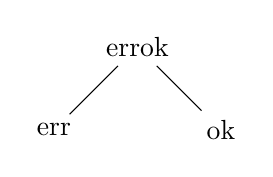
\begin{tikzpicture}[node distance=1.5cm]
    \node (top) at (0,0) {errok};
    \node [below left  of=top] (left)  {err};
    \node [below right of=top] (right) {ok};
    \draw (top) -- (left);
    \draw (top) -- (right);
  \end{tikzpicture}
\end{center}
Hinnangute osaline järjestusseos {\tt _⊑_} on toodud joonisel~\ref{fig:exc.ord}.
See seos on refleksiivne {\tt ⊑-refl}.
Transitiivsuse {\tt ⊑-trans} tõestus seisneb argumentide kuju juhtumi analüüsil.
Transitiivsuse seost on võimalik kodeerida järjestusseose konstruktorina, kuid see pole otstarbekas,
kuna hilisemates tõestuses tekib sellest täiendavad juhtumid, mida peab analüüsima.

\begin{figure}
  \begin{BVerbatim}
data _⊑_ : Exc → Exc → Set where
  ⊑-refl : {e : Exc} → e ⊑ e
  err⊑errok : err ⊑ errok
  ok⊑errok : ok ⊑ errok
  
⊑-trans : {e e' e'' : Exc} → e ⊑ e' → e' ⊑ e'' → e ⊑ e''
⊑-trans ⊑-refl q = q
⊑-trans err⊑errok ⊑-refl = err⊑errok
⊑-trans ok⊑errok ⊑-refl = ok⊑errok

_⊔_ : Exc → Exc → Exc
_⊓_ : Exc → Exc → Maybe Exc
⊔-sym : (e e' : Exc) → e ⊔ e' ≡ e' ⊔ e
⊓-sym : (e e' : Exc) → e ⊓ e' ≡ e' ⊓ e

lub : (e e' : Exc) → e ⊑ (e ⊔ e')
glb : (e e' : Exc) {e'' : Exc} → e ⊓ e' ≡ just e'' → e'' ⊑ e
lub-sym : (e e' : Exc) → e ⊑ (e' ⊔ e)
  \end{BVerbatim}
  \caption{Erandite efektide järjestus.}
  \label{fig:exc.ord}
\end{figure}
Loomulikul viisil saab defineerida erandi hinnangu ülemise ja alumise raja ning näidata nende sümmeetrilisust.
Lihtsuse huvides on toodud ainult vastavad tüübisignatuurid, aga mitte definitsioonid (jn~\ref{fig:exc.ord}).
Kuna kahel hinnangul ei pruugi leiduda alumine raja, siis on {\tt _⊓_} tulemus mähitud {\tt Maybe} monaadi.

\subsubsection{Eeljärjestatud monoid}\label{sssec:ordered-monoid}
Hulk {\tt E}, millel on defineeritud korrutamine {\tt _·_} ja ühikelement {\tt i},
st {\tt i} on ühik korrutamise suhtes nii vasakult {\tt lu} kui ka paremalt {\tt ru},
ning korrutamine on assotsiatiivne {\tt ass}, nimetatakse monoidiks.
Kui sellel hulgal on osaline järjestusseos {\tt _⊑_},
mis on refleksiivne {\tt ⊑-refl} ja transitiivne {\tt ⊑-trans},
ning kehtib korrutamise monotoonsus {\tt mon},
siis on tegemist eeljärjestatud monoidiga.
Joonisel~\ref{fig:ordered-monoid} on toodud eeljärjestatud monoidi kirje tüüp Agdas.

\begin{figure}
  \begin{BVerbatim}
record OrderedMonoid : Set where
  field
    E : Set
    _·_ : E → E → E    
    i : E

    lu : {e : E } → i · e ≡ e
    ru : {e : E } → e ≡ e · i 
    ass : {e e' e'' : E} → (e · e') · e'' ≡ e · (e' · e'')
    
    _⊑_ : E → E → Set    
    ⊑-refl : {e : E} → e ⊑ e
    ⊑-trans : {e e' e'' : E} → e ⊑ e' → e' ⊑ e'' → e ⊑ e''

    mon : {e e' e'' e''' : E} → e ⊑ e'' → e' ⊑ e''' → e · e' ⊑ e'' · e'''
  \end{BVerbatim}
  \caption{Eeljärjestatud monoid.}
  \label{fig:ordered-monoid}
\end{figure}

Saab näidata, et erandite efekti hinnag {\tt Exc},
korrutamine {\tt _·_}, mille ühikuks on konstruktor {\tt ok},
ja osaline järjestusseos {\tt _⊑_} moodustavad eeljärjestatud monoidi instantsi.
Vasakühiku tõestus tuleneb vahetult korrutamise definitsioonist.
Paremühiku tõestamisel tuleb teha juhtumi analüüs varjatud argumendi konstruktori kuju peal
ja seejärel lähtuda korrutamise definitsioonist.
Assotsiatiivsus tõestatakse sarnaselt kasutades juhtumite analüüsi ja korrutamise definitsiooni. Monotoonsuse tõestuses analüüsitakse nii võimalikke efekte kui ka nendevahelisi järjestusseoseid.
Kõik mainitud tõestused on toodud töö käigus valminud lähtekoodis.


\subsubsection{Gradeeritud monaad}\label{sssec:graded-monad}

Monaad on järgnev kolmik: tüübikonstruktor {\tt T}, tagastus {\tt η} ja sidumine {\tt bind}\footnote{Antud töös on {\tt bind}-i argumentide järjekord vahetunud võrreldes tavapärase käsitlusega.}.
\begin{equation*}
\begin{BVerbatim}
T : Set → Set
η : {X : Set} → X → T X
bind : {X Y : Set} → (X → T Y) → (T X → T Y)
\end{BVerbatim}
\end{equation*}
Seejuures peavad olema täidetud kolm monaadi seadust: vasakühik {\tt mlaw1}, paremühik {\tt mlaw2} ja assotsiatiivsus {\tt mlaw3}.
\begin{equation*}
\begin{BVerbatim}
mlaw1 : {X Y : Set} → (f : X → T Y) → (x : X) → bind f (η x) ≡ f x
mlaw2 : {X : Set} → (c : T X) → c ≡ bind η c
mlaw3 : {X Y Z : Set} → (f : X → T Y) → (g : Y → T Z) → (c : T X) →
        bind g (bind f c) ≡ bind (bind g ∘ f) c
\end{BVerbatim}
\end{equation*}

Joonisel~\ref{fig:graded-monad} on toodud eeljärjestatud monoidiga {\tt OM} gradeeritud monaadi kirje tüüp Agdas.
Efektiga {\tt E} parametriseeritud tüübikonstruktor {\tt T} koos tagastamisega {\tt η} ja sidumisega {\tt bind}  moodustab monaadi.
Neelduvusega {\tt sub} saab efektide järjestuse tõestusele tuginedes luua mingist monaadilisest väärtusest vastavalt suurema efektiga monaadilise väärtuse.
Neelduvus {\tt sub} peab olema refleksiivne {\tt sub-refl}, transitiivne {\tt sub-trans} ja  sidumise suhtes monotoonne {\tt sub-mon}.
Samuti peavad olema täidetud monaadi seadused {\tt mlaw1}, {\tt mlaw2} ja {\tt mlaw3}. Viimaste juures on kasutatud neelduvuse erijuhtu {\tt sub-eq} efektide võrdsuse korral pääsemaks mööda Agda tüübisüsteemist: ekvivalentsust ei saa tõestada eri tüüpi elementidele.

\begin{figure}
  \begin{BVerbatim}
subeq : {E : Set} → {T : E → Set → Set} → {e e' : E} → {X : Set} →
        e ≡ e' → T e X → T e' X
subeq refl p = p


record GradedMonad : Set where
  field
    OM : OrderedMonoid
  open OrderedMonoid OM
  field

    T : E → Set → Set
    η : {X : Set} → X → T i X
    bind : {e e' : E} {X Y : Set} → (X → T e' Y) → (T e X → T (e · e') Y)

    sub : {e e' : E} {X : Set} → e ⊑ e' → T e X → T e' X

    sub-mon : {e e' e'' e''' : E} {X Y : Set} →
              (p : e ⊑ e'') → (q : e' ⊑ e''') → 
              (f : X → T e' Y) → (c : T e X) → 
              sub (mon p q) (bind f c) ≡ bind (sub q ∘ f) (sub p c) 

  sub-eq : {e e' : E} {X : Set} → e ≡ e' → T e X → T e' X
  sub-eq = subeq {E} {T}
 
  field
    sub-refl : {e : E} {X : Set} → (c : T e X) → sub ⊑-refl c ≡ c
    sub-trans : {e e' e'' : E} {X : Set} →
                (p : e ⊑ e') → (q : e' ⊑ e'') → (c : T e X) → 
                sub q (sub p c) ≡ sub (⊑-trans p q) c   

    mlaw1 : {e : E} → {X Y : Set} → (f : X → T e Y) → (x : X) →
            sub-eq lu (bind f (η x)) ≡ f x
    mlaw2 : {e : E} → {X : Set} → (c : T e X) →
            sub-eq ru c ≡ bind η c
    mlaw3 : {e e' e'' : E} → {X Y Z : Set} →
            (f : X → T e' Y) → (g : Y → T e'' Z) → (c : T e X) → 
            sub-eq ass (bind g (bind f c)) ≡ bind (bind g ∘ f) c 
  \end{BVerbatim}
  \caption{Gradeeritud monaad.}
  \label{fig:graded-monad}
\end{figure}

Erandite järjestatud monoidi jaoks saab defineerida gradeeritud monaadi instantsi. Joonisel~\ref{fig:exc.graded-monad} on toodud olulisemad definitsioonid.
Tüübikonstruktor {\tt T} on defineeritud erandi hinnangu argumendi kuju järgi: veale {\tt err} vastab tipp-tüüp {\tt ⊤}, õnnestumisele {\tt ok} parameetriga antud tüüp {\tt X} ja hinnangule {\tt errok} vastab {\tt Maybe} monaad.
Ühikuks {\tt η} on identsusfunktsioon.
Sidumise {\tt bind} definitsioonil on analüüsitud kummagi efekti kuju ning vajadusel ka monaadilise väärtuse kuju.
Neelduvus {\tt sub} annab efektide refleksiivsuse {\tt ⊑-refl} korral monaadilise väärtuse {\tt c} enda.
Kui järjestuse tõestuse esimeseks efektis on {\tt err}, siis vastavalt tüübikonstruktori definitsioonile saab argument olla tipp-tüübi ainus element {\tt tt}, millele pannakse vastavusse {\tt nothing}.
Kui aga efektiks on {\tt ok}, siis vastav väärtus {\tt x} mähitakse {\tt Maybe} monaadi.

\begin{figure}
  \begin{BVerbatim}
T : Exc → Set → Set
T err X = ⊤
T ok X = X
T errok X = Maybe X

η : {X : Set} → X → T ok X
η x = x
  
bind : {e e' : Exc} {X Y : Set} →
       (X → T e' Y) → T e X → T (e · e') Y
bind {err} f x = tt
bind {ok} f x = f x
bind {errok} {err} f x = tt
bind {errok} {ok} f (just x) = just (f x)
bind {errok} {ok} f nothing = nothing
bind {errok} {errok} f (just x) = f x
bind {errok} {errok} f nothing = nothing

sub : {e e' : Exc} {X : Set} → e ⊑ e' → T e X → T e' X
sub ⊑-refl c = c
sub err⊑errok tt = nothing
sub ok⊑errok x = just x
  \end{BVerbatim}
  \caption{Osa erandite gradeeritud monaadi definitsioonist.}
  \label{fig:exc.graded-monad}
\end{figure}

\subsection{Tüübi- ja efektituletus}\label{ssec:exc.inference}

\subsubsection{Alamtüübid}\label{ssec:exc.subtypes}
Väärtus- ja arvutustüüpide osaline järjestus on vastastikku defineeritud (jn~\ref{fig:exc.subtypes}).
Konstruktoriga {\tt st-bn} loetakse tõeväärtused naturaalarvude alamtüübiks.
Kehtib väärtustüüpide refleksiivsus {\tt st-refl}.
Üks väärtustüübi paar on teise alamtüüp {\tt st-prod}, kui paaride vastavad projektsioonid on omakorda alamtüübid.
Funktsioonid on alamtüübid {\tt st-func}, kui funktsioonide kehade arvutused on alamtüübid,
ja funktsioonide argumendid on kontravariantsed.
Arvutustüüp on teise arvutustüübi alamtüüp {\tt st-comp}, kui nende efektid ja väärtustüübid on järjestatud.
\begin{figure}
  \begin{BVerbatim}
mutual
  data _≤V_ : VType → VType → Set where
    st-bn : bool ≤V nat
    st-refl : {σ : VType} → σ ≤V σ
    st-prod : {σ σ' τ τ' : VType} →
              σ ≤V σ' → τ ≤V τ' → σ ● τ ≤V σ' ● τ'
    st-func : {σ σ' : VType} {τ τ' : CType} →
              σ' ≤V σ → τ ≤C τ' → σ ⇒ τ ≤V σ' ⇒ τ'

  data _≤C_ : CType → CType → Set where
    st-comp : {e e' : E} {σ σ' : VType} →
              e ⊑ e' → σ ≤V σ' → e / σ ≤C e' / σ'

mutual
  st-trans : {σ σ' σ'' : VType} → σ ≤V σ' → σ' ≤V σ'' → σ ≤V σ''
  st-trans st-refl q = q
  st-trans p st-refl = p
  st-trans (st-prod p p') (st-prod q q') = st-prod (st-trans p q)
                                                   (st-trans p' q')
  st-trans (st-func p p') (st-func q q') = st-func (st-trans q p)
                                                   (sct-trans p' q')

  sct-trans : {σ σ' σ'' : CType} → σ ≤C σ' → σ' ≤C σ'' → σ ≤C σ''
  sct-trans (st-comp p q) (st-comp p' q') = st-comp (⊑-trans p p')
                                                    (st-trans q q')
  \end{BVerbatim}
  \caption{Väärtus- ja arvutustüüpide alamtüüpimine.}
  \label{fig:exc.subtypes}
\end{figure}

Väärtus- ja arvutustüüpide alamtüüpide transitiivsus on defineeritud vastastikku joonisel~\ref{fig:exc.subtypes}.
Kui väärtustüüpide transitiivsuse {\tt st-trans} üks argument on alamtüüpide refleksiivsuse {\tt st-refl} kujul, siis transitiivsus on määratud teise argumendiga.
Kui üks argument on alamtüüpide korrutise {\tt st-prod} kujul, siis ka teine argument peab olema paratamatult samal kujul. Sellisel juhul on transitiivsuseks alamtüüpide korrutis, mille korrutatavad on rekursiivselt määratud transitiivsusega {\tt st-trans}.
Kui üks argument on funktsiooni alamtüüpide {\tt st-func} kujul, siis on samal kujul ka teine argument. Transitiivsuseks on funktsiooni argumentide alamtüüpide kontravariantne transitiivsus {\tt st-trans} ja kehade arvutustüüpide transitiivsus {\tt sct-trans}.
Arvutustüüpide transitiivsuse {\tt sct-trans} argumendid saavad olla ainult arvutuste alamtüüpide {\tt st-comp} kujul. Vastav transitiivsus koostatakse arvutuste efektide järjestuse transitiivsusest {\tt ⊑-trans} ja väärtustüüpide transitiivsusest {\tt st-trans}.

\subsubsection{Rafineeritud keel}

Joonisel~\ref{fig:exc.refined} on toodud vastastikku defineeritud rafineeritud väärtus- ja arvutustermid.
Võrreldes alaptk~\ref{ssec:exc.raw}-s toodud termidega, on rafineeritud termid parametriseeritud kontekstiga {\tt Γ} ning indekseeritud vastavalt väärtus- ja arvutustüüpidega.
Kontekst {\tt Ctx} on defineeritud kui väärtusttüüpide list, mille elementide järjekord vastab vabade muutujate sissetoomise järjekorrale.
\begin{itemize}
\item Konstruktorid {\tt TT} ja {\tt FF} koostavad tõeväärtustüüpi termi.
\item Konstruktor {\tt ZZ} koostab naturaalarvu tüüpi termi. Konstruktor {\tt SS} koostab antud naturaalarvu tüüpi termi järglase, mis on samuti naturaalarvu tüüpi.
\item {\tt ⟨_,_⟩} koostab kahest antud väärtustermist paari, mille tüüp on termide tüüpide korrutis.
\item {\tt FST} ja {\tt SND} projekteerivad paari tüüpi termist vastavalt esimese või teise korrutatava tüüpi termi.
\item {\tt VAR} võtab tõestuse, et mingi tüüp on konteksti element, ning annab väärtustermi, mille tüüp on kõnealuse elemendiga määratud tüüp.
\item {\tt LAM} võtab väärtustüübi ja arvutustermi, mille kontekst on parameetriga antud kontekstist täpselt väärtustüübi argumendi võrra suurem, ning annab funktsiooniruumile vastava väärtustermi.
\item {\tt VCAST} suurendab ettantud väärtustermi tüüpi vastavalt alamtüübi tõestusele. See võimaldab erinevate alamtüüpidega väärtustermid ühtlustada, mis on vajalik rafineeritud arvutustermide koostamisel.
\end{itemize}

\begin{figure}
  \begin{BVerbatim}
Ctx = List VType

mutual
 data VTerm (Γ : Ctx) : VType → Set where
   TT FF : VTerm Γ bool
   ZZ : VTerm Γ nat
   SS : VTerm Γ nat → VTerm Γ nat
   ⟨_,_⟩ : {σ σ' : VType} →
           VTerm Γ σ → VTerm Γ σ' → VTerm Γ (σ ● σ')
   FST : {σ σ' : VType} → VTerm Γ (σ ● σ') → VTerm Γ σ
   SND : {σ σ' : VType} → VTerm Γ (σ ● σ') → VTerm Γ σ'
   VAR : {σ : VType} → σ ∈ Γ → VTerm Γ σ
   LAM : (σ : VType) {τ : CType} →
         CTerm (σ ∷ Γ) τ → VTerm Γ (σ ⇒ τ)
   VCAST : {σ σ' : VType} → VTerm Γ σ → σ ≤V σ' → VTerm Γ σ'

 data CTerm (Γ : Ctx) : CType → Set where
   VAL : {σ : VType} → VTerm Γ σ → CTerm Γ (ok / σ)
   FAIL : (σ : VType) → CTerm Γ (err / σ)
   TRY_WITH_ : {e e' : E} {σ : VType} → CTerm Γ (e / σ) →
               CTerm Γ (e' / σ) → CTerm Γ (e ⊹ e' / σ)
   IF_THEN_ELSE_ : {e e' : E} {σ : VType} → VTerm Γ bool →
                CTerm Γ (e / σ) → CTerm Γ (e' / σ) → CTerm Γ (e ⊔ e' / σ)
   _$_ : {σ : VType} {τ : CType} →
         VTerm Γ (σ ⇒ τ) → VTerm Γ σ → CTerm Γ τ
   PREC : {e e' : E} {σ : VType} → VTerm Γ nat →
          CTerm Γ (e / σ) → CTerm (σ ∷ nat ∷ Γ) (e' / σ) →
          e · e' ⊑ e → CTerm Γ (e / σ)
   LET_IN_ : {e e' : E} {σ σ' : VType} → CTerm Γ (e / σ) →
             CTerm (σ ∷ Γ) (e' / σ') → CTerm Γ (e · e' / σ')
   CCAST : {e e' : E} {σ σ' : VType} → CTerm Γ (e / σ) →
           e / σ ≤C e' / σ' → CTerm Γ (e' / σ')
  \end{BVerbatim}
  \caption{Eranditega keele rafineeritud termid.}
  \label{fig:exc.refined}
\end{figure}

Rafineeritud arvutustermid (jn~\ref{fig:exc.refined}) määravad täpselt osaarvutuste efektide kombineerimise.
\begin{itemize}
\item {\tt VAL} koostab antud väärtustermist õnnestunud arvutuse.
\item {\tt FAIL} koostab väärtustüübist ebaõnnestunud arvutuse.
\item {\tt TRY_WITH_} parandab põhiarvutustermi efekti erandikäsitleja arvutustermi efektiga. Kitsendusena peavad arvutustermid omama sama väärtustüüpi.
\item {\tt IF_THEN_ELSE_} eeldab tõeväärtustüüpi tingimust. Kogu arvutustermi efekt on määratud harude, millede väärtustüübid peavad ühtima, efektide ülemise rajaga.
\item {\tt _\$_} rakendab esimesega väärtustermiga antud funktsiooni teise väärtustermiga argumendile, seejuures peavad funktsiooni parameetri ja argumendi väärtustüübid ühtima. Kogu arvutuse efekt ja väärtustüüp on määratud funktsiooni keha arvutustüübiga. 
\item {\tt PREC} eeldab sammude arvuna naturaalarvude tüüpi väärtustermi. Baasarvutuse väärtustüüp on lisatud koos naturaalarvu tüüpi sammuloenduriga sammu arvutustermi konteksti. Täiendava kitsendusena on nõutud, et baasi efekt oleks sammu efektiga korrutamisel püsipunkt.
\item {\tt LET_IN_} lisab esimese arvutustermi väärtustüübi teise arvutustermi konteksti. Kogu arvutuse efektis on arvutustermide korrutis ning väärtustüüp on määratud teise arvutustermi tüübiga.
\item {\tt CCAST} suurendab etteantud arvutustermi tüüpi vastavalt alamtüübi tõestusele.
\end{itemize}


\subsubsection{Termide tüübituletus}\label{sssec:exc.infer-type}

Etteantud kontekstis saab väärtustermile tuletada vastava väärtustüübi (jn~\ref{fig:exc.infer-vtype}).
Kuna vaste võib puududa, siis on {\tt infer-vtype} tulemus mähitud {\tt Maybe} monaadi.
Väärtustüübi tuletamisel lähtutakse väärtustüübi konstruktori kujust.
\begin{itemize}
\item {\tt TT} ja {\tt FF} annavad kindlasti tõeväärtustüübi.
\item {\tt ZZ} on kindlasti naturaalarvu tüüpi. {\tt SS t} korral tuleb täiendavalt kontrollida, kas alamterm {\tt t} on samas kontekstis naturaalarvu tüüpi. Vastasel korral on term halvasti koostatud ja selle tüüp puudub.
\item Paari {\tt ⟨ t , t' ⟩} tüüp on määratud, kui alamtermide {\tt t} ja {\tt t'} tüübid on samas kontekstis määratud. Paari tüübiks on alamtermide tüüpide korrutis. Ülejäänud juhtudel pole paari tüüp määratud.
\item {\tt FST t} ja {\tt SND t} on määratud, kui alamterm {\tt t} on paar, st antud kontekstis on ta korrutise tüüpi. Projektsiooni tüübiks on vastavalt esimene või teine korrutatav.
\item {\tt VAR x} korral tuleb kontrollida, et naturaalarv {\tt x} on väiksem kui kontekst {\tt Γ} pikkus. Selleks on kasutatud lahendajat {\tt _<?_}. Naturaalarvude võrratusest {\tt p} on koostatud konteksti pikkusega piiratud naturaalarv {\tt fromℕ≤ p}, mida kasutatakse muutujale vastava tüübi otsimiseks kontekstist {\tt lkp Γ}.
\item {\tt LAM σ t} puhul tuleb kontrollida, et arvutustermiga {\tt t} antud keha on hästi tüübitud kontekstis, mida on laiendatud parameetri {\tt σ} võrra. Arvutustermi tüübituletus {\tt infer-ctype} on toodud allpool.
\end{itemize}

\begin{figure}
  \begin{BVerbatim}
infer-vtype : Ctx → vTerm → Maybe VType
infer-vtype Γ TT = just bool
infer-vtype Γ FF = just bool
infer-vtype Γ ZZ = just nat
infer-vtype Γ (SS t) with  infer-vtype Γ t
... | just nat = just nat
... | _        = nothing
infer-vtype Γ ⟨ t , t' ⟩ with infer-vtype Γ t | infer-vtype Γ t'
... | just σ | just σ' = just (σ ● σ')
... | _      | _       = nothing
infer-vtype Γ (FST t) with infer-vtype Γ t
... | just (σ ● _) = just σ
... | _            = nothing
infer-vtype Γ (SND t) with infer-vtype Γ t
... | just (_ ● σ') = just σ'
... | _             = nothing
infer-vtype Γ (VAR x) with x <? Γ
... | yes p = just (lkp Γ (fromℕ≤ p))
... | no ¬p = nothing
infer-vtype Γ (LAM σ t) with infer-ctype (σ ∷ Γ) t
... | just τ = just (σ ⇒ τ)
... | _      = nothing
  \end{BVerbatim}
  \caption{Eranditega keele väärtustermide tüübituletus.}
  \label{fig:exc.infer-vtype}
\end{figure}

Joonisel~\ref{fig:exc.infer-ctype} on toodud etteantud kontekstis arvutustermile tüübi tuletamine.
Nagu väärtustermide tüübituletuse puhul, on ka arvutustermide tüübituletus {\tt infer-ctype} tulemus mähitud {\tt Maybe} monaadi.
Väärtustüübi tuletamisel lähtutakse väärtustüübi konstruktori kujust.
\begin{itemize}
\item {\tt VAL x} on tüübitud, kui väärtustermi {\tt x} tüübituletus õnnestub. Arvutuse väärtustüübiks on tuletatud tüüp. Efekti hinnang {\tt ok} tähistab arvutuse õnnestumist. 
\item {\tt FAIL σ} on alati väärtustüübi {\tt σ} ebaõnnestumise tüüpi, mille efekti hinnang on {\tt err}.
\item {\tt TRY t WITH t'} on tüübitud, kui arvutustermid {\tt t} ja {\tt t'} on hästi tüübitud. Kogu arvutuse tüübiks on põhiarvutuse tüübi {\tt τ} parandamine erandikäsitleja tüübiga {\tt τ'}. Arvutustüüpide parandus _⊹C_ on defineeritud efektide paranduse _⊹_ ja väärtustüüpide ülemise raja _⊔V_ abil.
\item {\tt IF x THEN t ELSE t'} eeldab, et väärtusterm {\tt x} on tõeväärtustüüpi. Kogu arvutuse tüüp on määratud harude tüüpide {\tt τ} ja {\tt τ'} ülemise rajaga {\tt τ ⊔C τ'}.
\item {\tt f \$ t} korral kontrollitakse, et väärtustermi {\tt f} tüübiks on funktsiooniruum ja väärtustermile {\tt t} tuletatud tüüp on {\tt f} parameetri alamtüüp. Ülejäänud juhtudel ei ole funktsiooni rakendamine hästi tüübitud.
\item {\tt PREC x t t'} korral kontollitakse viit tingimust.
  \begin{itemize}
  \item Väärtusterm {\tt x} peab olema antud kontekstis naturaalarvu tüüpi.
  \item Baasi arvutusterm {\tt t} peab olema antud kontekstis hästi tüübitud.
  \item Sammu arvutusterm {\tt t'} peab olema tüübitud kontekstis, kuhu on lisatud naturaalarvu tüübi sammuloendur ja arvutustermi {\tt t} väärtustüüpi {\tt σ} akumulaator.
  \item Osaarvutustele tuletatud väärtustüübid peavad olema samad. Selleks kasutatakse lahendajat {\tt _≡V?_}.
  \item Osaarvutuste efektide korrutis ei tohi olla suurem, kui baasi efekt. Seda kontrollitakse lahendajaga {\tt _⊑?_}.
  \end{itemize}
  Kui kõik tingimused kehtivad, siis kogu arvutuse tüüp on määratud baasi efekti ja väärtustüübiga.
\item {\tt LET t IN t'} on tüübitud, kui arvutusterm {\tt t} on tüübitud antud kontekstis ja arvutusterm {\tt t'} on tüübitud kontekstis, mida on laiendatud esimese osaarvutuse väärtustüübi võrra. Arvutuse efektiks on osarvutuste efektide korrutis ning väärtustüübiks teise osaarvutuse väärtustüüp. Kui üks osaarvutust ei ole hästi tüübitud, siis ei ole ka kogu arvutus tüübitud.
\end{itemize}

\begin{figure}
  \begin{BVerbatim}
infer-ctype : Ctx → cTerm → Maybe CType
infer-ctype Γ (VAL x) with infer-vtype Γ x
... | just σ = just (ok / σ)
... | _      = nothing
infer-ctype Γ (FAIL σ) = just (err / σ)
infer-ctype Γ (TRY t WITH t') with infer-ctype Γ t | infer-ctype Γ t'
... | just τ | just τ' = τ ⊹C τ'
... | _      | _       = nothing
infer-ctype Γ (IF x THEN t ELSE t')
    with infer-vtype Γ x | infer-ctype Γ t | infer-ctype Γ t'
... | just bool | just τ | just τ' = τ ⊔C τ'
... | _         | _      | _       = nothing
infer-ctype Γ (f $ t) with infer-vtype Γ f | infer-vtype Γ t
... | just (σ ⇒ τ) | just σ' with σ' ≤V? σ
...                           | yes _ = just τ
...                           | no  _ = nothing
infer-ctype Γ (f $ t) | _ | _ = nothing
infer-ctype Γ (PREC x t t')
    with infer-vtype Γ x
... | just nat with infer-ctype Γ t
...        | nothing = nothing
...        | just (e / σ) with infer-ctype (σ ∷ nat ∷ Γ) t'
...                       | nothing = nothing
...                       | just (e' / σ') with e · e' ⊑? e | σ ≡V? σ'
...                                        | yes _ | yes _ = just (e / σ)
...                                        | _     | _     = nothing
infer-ctype Γ (PREC x t t') | _ = nothing
infer-ctype Γ (LET t IN t') with infer-ctype Γ t 
... | nothing = nothing
... | just (e / σ) with infer-ctype (σ ∷ Γ) t'
...                | nothing        = nothing
...                | just (e' / σ') = just (e · e' / σ')
  \end{BVerbatim}
  \caption{Eranditega keele arvutustermide tüübituletus.}
  \label{fig:exc.infer-ctype}
\end{figure}

\subsubsection{Termide rafineerimine}

Kui n-ö ``toorele'' termile õnnestub mingis kontekstis tuletada tüüp, siis saab sellest termist konstrueerida rafineeritud termi.
Joonisel~\ref{fig:exc.infer-term-type} on toodud väärtus- ja arvutustermide rafineeritud tüübikonstruktorid.
Tipp-tüüp {\tt ⊤} tähistab tüübituletuse ebaõnnestumist.
\begin{figure}
  \begin{BVerbatim}
refined-vterm : Ctx → vTerm → Set
refined-vterm Γ t with infer-vtype Γ t 
... | nothing = ⊤
... | just τ = VTerm Γ τ

refined-cterm : Ctx → cTerm → Set
refined-cterm Γ t with infer-ctype Γ t 
... | nothing = ⊤
... | just τ = CTerm Γ τ
  \end{BVerbatim}
  \caption{Väärtus- ja arvutustermide rafineerimiste tüübikonstruktorid.}
  \label{fig:exc.infer-term-type}
\end{figure}

Väärtustermide rafineerimine etteantud kontekstis (jn~\ref{fig:exc.refine-vterm}) matkib väärtustermide tüübituletust (alaptk~\ref{sssec:exc.infer-type}).
\begin{itemize}
\item {\tt TT} ja {\tt FF} korral konstrueeritakse vastav rafineeritud väärtusterm.
\item {\tt ZZ} puhul konstrueeritakse rafineeritud väärtusterm null {\tt ZZ}. {\tt SS t} korral kontrollitakse, et väärtusterm {\tt t} on hästi tüübitud ja on naturaalarvu tüüpi. Rafineeritud naturaalarvu järglane {\tt SS} koostatakse alamväärtuse {\tt t} rafineeringust {\tt u}. Kui väärtustermi {\tt t} tüübituletus ei õnnestu või tuletatud tüüp ei ole naturaalarvu tüüpi, siis rafineeringu tulemuseks koostatakse tipp-tüübi element {\tt tt}.
\item {\tt ⟨ t , t' ⟩} korral kontrollitakse, et mõlemad väärtustermid {\tt t} ja {\tt t'} on kontekstis hästi tüübitud ja rafineeritud paar koostatakse rafineeritud termidest {\tt u} ja {\tt u'}.
\item {\tt FST t} puhul peab väärtustermile {\tt t} tuletatud tüüp olema korrutis. Rafineeritud projektsiooni saab koostada {\tt t} rafineeringust {\tt u}. {\tt SND t} juhtum on analoogne.
\item {\tt VAR x} korral koostatakse lahendist {\tt p}, mis näitab, et naturaalarv {\tt x} on väiksem kui konteksti {\tt Γ} pikkus, rafineeritud muutuja tõestusega, et {\tt x}-iga määratud muutuja on kontekstis.
\item {\tt LAM σ t} juhtumis lisatakse parameetri tüüp {\tt σ} konteksti ja kontrollitakse arvutustermi {\tt t} hästi-tüübitust. Rafineeritud funktsiooni abstraktsioon koostatakse uues kontekstis rafineeritud arvutusest {\tt u}.
\end{itemize}

\begin{figure}
  \begin{BVerbatim}
refine-vterm : (Γ : Ctx) (t : vTerm) → refined-vterm Γ t 
refine-vterm Γ TT = TT
refine-vterm Γ FF = FF
refine-vterm Γ ZZ = ZZ
refine-vterm Γ (SS t) with infer-vtype Γ t | refine-vterm Γ t
... | just nat | u = SS u
... | just bool | _ = tt
... | just (_ ● _) | _ = tt
... | just (_ ⇒ _) | _ = tt
... | nothing | _ = tt
refine-vterm Γ ⟨ t , t' ⟩
    with infer-vtype Γ t | refine-vterm Γ t |
         infer-vtype Γ t' | refine-vterm Γ t'
... | just _  | u | just _  | u' = ⟨ u , u' ⟩
... | just _  | _ | nothing | _  = tt
... | nothing | _ | _       | _  = tt
refine-vterm Γ (FST t) with infer-vtype Γ t | refine-vterm Γ t
... | just nat | _ = tt
... | just bool | _ = tt
... | just (_ ● _) | u = FST u
... | just (_ ⇒ _) | _ = tt
... | nothing | _ = tt
refine-vterm Γ (SND t) with infer-vtype Γ t | refine-vterm Γ t
... | just nat | _ = tt
... | just bool | _ = tt
... | just (_ ● _) | u = SND u
... | just (_ ⇒ _) | _ = tt
... | nothing | _ = tt
refine-vterm Γ (VAR x) with x <? Γ
... | yes p = VAR (trace Γ (fromℕ≤ p))
... | no _  = tt
refine-vterm Γ (LAM σ t)
    with infer-ctype (σ ∷ Γ) t | refine-cterm (σ ∷ Γ) t
... | just _ | u = LAM σ u
... | nothing | u = tt
  \end{BVerbatim}
  \caption{Eranditega keele väärtustermide rafineerimine.}
  \label{fig:exc.refine-vterm}
\end{figure}

Arvutustermide rafineerimine on toodud joonistel~\ref{fig:exc.refine-cterm1} ja~\ref{fig:exc.refine-cterm2}.
\begin{itemize}
\item {\tt VAL t} korral kontrollitakse, et väärtusterm {\tt t} on hästi tüübitud, ja rafineeritud arvutus koostatakse vastavast rafineeritud väärtustermist {\tt u}.
\item {\tt FAIL σ} rafineerimisel näidatakse, et selle arvutustermi tüübituletus alati õnnestub.
\item {\tt TRY t WITH t'} korral kontrollitakse, et mõlemad osaarvutused on hästi tüübitud ja tuletatud väärtustüüpidel leidub ülemine raja. Rafineeritud arvutuse konstrueerimiseks suurendatakse rafineeritud osaarvutuste {\tt u} ja {\tt u'} tüüpi ülemise rajani vastavalt alamtüübi tõestusele {\tt p}.
\item {\tt IF x THEN t ELSE t'} korral peab väärtusterm {\tt x} olema tõeväärtustüüpi ning arvutustermid {\tt t} ja {\tt t'} peavad olema hästi tüübitud. Kui harude arvutuste väärtustüüpidel leidub ülemine raja, siis rafineeritud tingimuslause tingimus on rafineeritud väärtusterm {\tt x'} ja tingimuslause harudes suurendatakse rafineeritud arvutuste {\tt u} ja {\tt u'} tüüpi vastavalt alamtüübi tõestusele {\tt p}. Ülejäänud juhtudel koostatakse tipp-tüübi element {\tt tt}.
\item {\tt f \$ x} korral peab väärtusterm {\tt f} olema funktsiooniruumi tüüpi ja seejuures peab argumendile {\tt x} tuletatud tüüp olema mainitud funktsiooniruumi parameetri alamtüüp. Rafineeritud funktsiooni {\tt f'} rakendamise koostamisel on rafineeritud argumendi {\tt x'} tüüpi suurendatud vastavalt alamtüübi tõestusele {\tt p}.
\item {\tt PREC x t t'} korral kontrollitakse, et väärtusterm {\tt x} on naturaalarvu tüüpi ning baasile vastav arvutus {\tt t} hästi tüübitud. Seejärel, et sammule vastav arvutus {\tt t'} on hästi tüübitud kontekstis, kuhu on lisatud naturaalarvu tüüpi sammuloendur ning baasi väärtustüübile vastav akumulaator. Viimaks kontrollitakse, et baasi ja sammu efektide korrutamine ei ületaks baasi efekti ning et baasile ja sammule vastavad väärtustüübid langevad kokku. Rafineeritud primitiivse rekursiooni term koostatakse vastavatest rafineeritud termidest {\tt x'}, {\tt u}, {\tt u'} ja efektide püsipunkti tõestusest {\tt p}.
\item {\tt LET t IN t'} puhul peab osaarvutus {\tt t} olema hästi tüübitud antud kontekstis ja osaarvutus {\tt t'} tüübitud kontekstis, kuhu on lisatud {\tt t}-le tuletatud tüüp {\tt σ}. Rafineeritud arvutuste sidumine koostatakse rafineeritud osaarvutustest {\tt u} ja {\tt u'}.
\end{itemize}
\begin{figure}
  \begin{BVerbatim}
refine-cterm : (Γ : Ctx) (t : cTerm) → refined-cterm Γ t
refine-cterm Γ (VAL t) with infer-vtype Γ t | refine-vterm Γ t
... | nothing | u = tt
... | just _ | u = VAL u
refine-cterm Γ (FAIL σ) with infer-ctype Γ (FAIL σ)
... | _ = FAIL σ
refine-cterm Γ (TRY t WITH t')
    with infer-ctype Γ t | refine-cterm Γ t |
         infer-ctype Γ t' | refine-cterm Γ t'
... | nothing      | _ | _              | _ = tt
... | just _       | _ | nothing        | _ = tt
... | just (e / σ) | u | just (e' / σ') | u'
         with σ ⊔V σ' | inspect (_⊔V_ σ) σ'
...      | nothing | _ = tt
...      | just _ | [ p ] =
    TRY  CCAST u (⊔V-subtype p)
    WITH CCAST u' (⊔V-subtype-sym {σ} p)
refine-cterm Γ (IF x THEN t ELSE t')
    with infer-vtype Γ x | refine-vterm Γ x
... | nothing | _ = tt
... | just nat | _ = tt
... | just (_ ● _) | _ = tt
... | just (_ ⇒ _) | _ = tt
... | just bool | x'
         with infer-ctype Γ t | refine-cterm Γ t
...      | nothing | u = tt
...      | just (e  / σ) | u
              with infer-ctype Γ t' | refine-cterm Γ t'
...           | nothing | u' = tt
...           | just (e' / σ') | u'
                   with σ ⊔V σ' | inspect (_⊔V_ σ) σ'
...                | nothing | _     = tt
...                | just ⊔σ | [ p ] =
    IF x' THEN CCAST u (⊔V-subtype p)
          ELSE CCAST u' (⊔V-subtype-sym {σ} p)
--
  \end{BVerbatim}
  \caption{Eranditega keele arvutustermide rafineerimine, I osa.}
  \label{fig:exc.refine-cterm1}
\end{figure}
\begin{figure}
  \begin{BVerbatim}
--refine-cterm : (Γ : Ctx) (t : cTerm) → refined-cterm Γ t
refine-cterm Γ (f $ x)
    with infer-vtype Γ f | refine-vterm Γ f |
         infer-vtype Γ x | refine-vterm Γ x
... | nothing   | _ | _ | _ = tt
... | just nat  | _ | _ | _ = tt
... | just bool | _ | _ | _ = tt
... | just (_ ● _) | _ | _ | _ = tt
... | just (_ ⇒ _) | _ | nothing | _ = tt  
... | just (σ ⇒ τ) | f' | just σ' | x' with σ' ≤V? σ
...                                    | no _  = tt
...                                    | yes p = f' $ VCAST x' p
refine-cterm Γ (PREC x t t')  with infer-vtype Γ x | refine-vterm Γ x
... | nothing | _  = tt
... | just bool | _ = tt
... | just (_ ● _) | _ = tt
... | just (_ ⇒ _) | _ = tt
... | just nat | x'
        with infer-ctype Γ t | refine-cterm Γ t 
...     | nothing | _ = tt
...     | just (e / σ) | u
            with infer-ctype (σ ∷ nat ∷ Γ) t' |
                 refine-cterm (σ ∷ nat ∷ Γ) t'
...         | nothing | _ = tt
...         | just (e' / σ') | u' with e · e' ⊑? e | σ ≡V? σ'
...                               | no  _ | _    = tt
...                               | yes _ | no _ = tt
refine-cterm Γ (PREC x t t')
    | just nat | x'
        | just (e / σ) | u
            | just (e' / .σ) | u' | yes p | yes refl = PREC x' u u' p
refine-cterm Γ (LET t IN t') with infer-ctype Γ t | refine-cterm Γ t 
... | nothing | _  = tt
... | just (e / σ) | u with infer-ctype (σ ∷ Γ) t' |
                            refine-cterm (σ ∷ Γ) t'
...                    | nothing        | _  = tt
...                    | just (e' / σ') | u' = LET u IN u'
  \end{BVerbatim}
  \caption{Eranditega keele arvutustermide rafineerimine, II osa.}
  \label{fig:exc.refine-cterm2}
\end{figure}

\subsection{Semantika}\label{ssec:exc.semantics}

Joonisel~\ref{fig:type-semantics} on toodud vastastikku defineeritud väärtus- ja arvutustüüpide ning konteksti semantiline interpretatsioon metakeeles Agda.
\begin{itemize}
\item {\tt nat} interpreteeritakse kui naturaalarvud {\tt ℕ} ja {\tt bool} kui tõeväärtused {\tt Bool}.
\item {\tt σ ● σ'} korral tehakse rekursiivsed väljakutsed korrutatavatele ning tulemused korrutatakse Agdas {\tt _×_}.
\item {\tt σ ⇒ τ} interpretatsioon vastab Agda funktsioonile, mille parameetri ja tulemuse tüüp on interpreeritud vastavalt väärtustüübist {\tt σ} ja arvutustüübist {\tt τ}.
\item Arvutustüübi {\tt ε / σ} interpreteerimiseks rakendatakse gradeeritud monaadi tüübikonstruktorit {\tt T} efektile {\tt ε} ja väärtustüübi {\tt σ} interpretatsioonile.
\item Tühi kontekst vastab tipp-tüübile {\tt ⊤}. Mitte-tühja konteksti pea-element interpreteeritakse ja korrutatakse rekursiivselt interpreteeritud sabaga.
\end{itemize}

\begin{figure}
  \begin{BVerbatim}
mutual
  ⟪_⟫V : VType → Set
  ⟪ nat ⟫V = ℕ
  ⟪ bool ⟫V = Bool
  ⟪ σ ● σ' ⟫V = ⟪ σ ⟫V × ⟪ σ' ⟫V
  ⟪ σ ⇒ τ ⟫V = ⟪ σ ⟫V → ⟪ τ ⟫c

  ⟪_⟫c : CType → Set
  ⟪ ε / σ ⟫c = T ε ⟪ σ ⟫V

⟪_⟫X : Ctx → Set
⟪ [] ⟫X = ⊤
⟪ σ ∷ Γ ⟫X = ⟪ σ ⟫V × ⟪ Γ ⟫X
  \end{BVerbatim}
  \caption{Väärtus-, arvutustüüpide ja konteksti semantika.}
  \label{fig:type-semantics}
\end{figure}

Joonisel~\ref{fig:exc.vterm-semantics} on toodud rafineeritud väärtustermi interpretatsioon antud konteksti interpretatsioonis.
\begin{itemize}
\item {\tt TT} ja {\tt FF} seatakse vastavusse tõese ja vääraga.
\item {\tt ZZ} vastab nullile. {\tt SS t} on {\tt t} interpretatsiooni järglane.
\item {\tt ⟨ t , t' ⟩} tõlgendatakse kui {\tt t} ja {\tt t'} interpretatsioonide paari.
\item {\tt FST t} ja {\tt SND t} teevad vastavalt esimese ja teise projektsiooni {\tt t} interpretatsioonist.
\item {\tt VAR x} projekteerib konteksti interpretatsioonist {\tt ρ} tõestusele {\tt x} vastava (n-ö {\tt x}-nda) väärtuse.
\item {\tt LAM σ t} interpreteeritakse kui lambda abstraktsiooni, mille seotud muutuja {\tt x} lisatakse arvutustermi {\tt t} interpreteerimise konteksti.
\item {\tt VCAST t p} puhul interpreteeritakse väärtusterm {\tt t} ja konverteeritakse see vastavalt alamtüübi tõestusele {\tt p}.
\end{itemize}

\begin{figure}
  \begin{BVerbatim}
⟦_⟧V : {Γ : Ctx} {σ : VType} → VTerm Γ σ → ⟪ Γ ⟫X → ⟪ σ ⟫V
⟦ TT ⟧V ρ = true
⟦ FF ⟧V ρ = false
⟦ ZZ ⟧V ρ = zero
⟦ SS t ⟧V ρ = suc (⟦ t ⟧V ρ)
⟦ ⟨ t , t' ⟩ ⟧V ρ = ⟦ t ⟧V ρ , ⟦ t' ⟧V ρ
⟦ FST t ⟧V ρ = proj₁ (⟦ t ⟧V ρ)
⟦ SND t ⟧V ρ = proj₂ (⟦ t ⟧V ρ)
⟦ VAR x ⟧V ρ = proj x ρ
⟦ LAM σ t ⟧V ρ = λ x → ⟦ t ⟧C (x , ρ)
⟦ VCAST t p ⟧V ρ = vcast p (⟦ t ⟧V ρ)
  \end{BVerbatim}
  \caption{Eranditega keele väärtustermide semantika.}
  \label{fig:exc.vterm-semantics}
\end{figure}

Rafineeritud arvutustermi semantiline interpretatsioon etteantud konteksti interpretatsioonis on toodud joonisel~\ref{fig:exc.cterm-semantics}.
\begin{itemize}
\item {\tt VAL x} interpreteerib väärtustermi {\tt x} antud kontekstis ja tagastab selle gradeeritud monaadis.
\item Kuna arvutustüübi, mille efekt on {\tt err}, interpretatsioon erandite gradeeritud monaadis on tipp-tüüp {\tt ⊤}, siis {\tt FAIL σ} koostab selle ainsa elemendi {\tt tt}.
\item {\tt TRY_WITH_ {e} {e'} t t'} kombineerib osaarvutuste {\tt t} ja {\tt t'} interpretatsioonid vastavalt arvutuste efektidele. Semantiline erandikäsitlus {\tt or-else} käitub järgnevalt. Kui esimese osaarvutuse efektiks on ebaõnnestumine {\tt err}, siis kogu arvutus on määratud erandikäsitlejaga. Kui esimene arvutus õnnestub efektiga {\tt ok}, siis kogu arvutuseks ongi esimene arvutus. Kui esimese arvutuse õnnestumine pole teada, st efektiks on {\tt errok}, siis analüüsitakse ka erandikäsitleja efekti. Kui erandikäsitleja efekt on {\tt err}, siis on kogu arvutus määratud põhiarvutusega. Ülejäänud juhtudel analüüsitakse esimese arvutuse tulemuse kuju: kui esimene arvutus ikkagi õnnestus (konstruktor {\tt just}), siis saab sealt ka kogu arvutuse tulemuse; vastasel korral on kogu arvutuse tulemuseks erandikäsitleja tulemus.
\item {\tt IF_THEN_ELSE_} korral interpreteeritakse tingimus ja harud tingimuslauses, kusjuures kummagi haru efekt neeldub efektide ülemises rajas.
\item {\tt PREC x t t' p} interpretatsioon vastab primitiivsele rekursioonile, mille sammude arv on on väärtustermi {\tt x} interpretatsioon, baas on arvutustermi {\tt t} interpretatsioon ja sammuks on arvutustermi {\tt t'} interpretatsioon kontekstis, kuhu on lisatud sammuloendur ja vahetulemuse akumulaator. Semantiline primitiivne rekursioon {\tt primrecT} on defineeritud induktsiooniga sammude arvul. Nulli korral on tulemuseks baasile vastav arvutus {\tt z}. Sammu korral rakendatakse sammule vastavat funktsiooni {\tt s} sammuloendurile {\tt n} ja saadud funktsioon seotakse {\tt bind}-iga rekursiive väljakutsega. Tulemuse efekt neeldub efektide püsipunkti tõestuse {\tt p} tõttu baasarvutuse efektis.
\item {\tt f \$ x} korral rakendatakse väärtustermi {\tt f} interpretatsiooni väärtustermi {\tt x} interpretatsioonile.
\item {\tt LET_IN_} seob osaarvutused: esimese osarvutuse interpretatsioon lisatakse teise osaarvutuse interpreteerimise konteksti.
\item {\tt CCAST t p} puhul interpreteeritakse arvutusterm {\tt t} ja konverteeritakse see vastavalt alamtüübi tõestusele {\tt p}.
\end{itemize}

\begin{figure}
  \begin{BVerbatim}
or-else : (e e' : E) {X : Set} → T e X → T e' X → T (e ⊹ e') X
or-else err _ _ x' = x'
or-else ok _ x _ = x
or-else errok err x _ = x
or-else errok ok (just x) _ = x
or-else errok ok nothing x' = x'
or-else errok errok (just x) x' = just x
or-else errok errok nothing x' = x'

primrecT : {e e' : E} {X : Set} →
           ℕ → T e X → (ℕ → X → T e' X) → e · e' ⊑ e → T e X
primrecT zero z s p = z
primrecT {e} {e'} (suc n) z s p =
    sub p (bind {e} {e'} (s n) (primrecT n z s p))

⟦_⟧C : {Γ : Ctx} {τ : CType} → CTerm Γ τ → ⟪ Γ ⟫X → ⟪ τ ⟫c
⟦ VAL x ⟧C ρ = η (⟦ x ⟧V ρ)
⟦ FAIL σ ⟧C ρ = tt
⟦ TRY_WITH_ {e} {e'} t t' ⟧C ρ = or-else e e' (⟦ t ⟧C ρ) ( (⟦ t' ⟧C ρ))
⟦ IF_THEN_ELSE_ {e} {e'} x t t' ⟧C ρ = if ⟦ x ⟧V ρ
                                      then (sub (lub e e') (⟦ t ⟧C ρ))
                                      else (sub (lub-sym e' e) (⟦ t' ⟧C ρ))
⟦ PREC x t t' p ⟧C ρ = primrecT (⟦ x ⟧V ρ) (⟦ t ⟧C ρ)
                                ((λ i acc → ⟦ t' ⟧C (acc , i , ρ))) p
⟦ f $ x ⟧C ρ = ⟦ f ⟧V ρ (⟦ x ⟧V ρ)
⟦ LET_IN_ {e} {e'} m n ⟧C ρ =
    bind {e} {e'} (λ x → ⟦ n ⟧C (x , ρ)) (⟦ m ⟧C ρ)
⟦ CCAST t o ⟧C ρ = ccast o (⟦ t ⟧C ρ)
  \end{BVerbatim}
  \caption{Eranditega keele arvutustermide semantika.}
  \label{fig:exc.cterm-semantics}
\end{figure}

\subsection{Optimisatsioonid}\label{ssec:exc.optimizations}

Etteantud kontekstist saab jätta välja selle mingis kohas oleva tüübi, eeldusel, et sellele vastavat muutujat pole üheski termis tarvis.
Seda nimetatakse konteksti lõdvendamiseks {\tt dropX} (jn~\ref{fig:weakening}).
Samamoodi saab lõdvendada rafineeritud väärtusterme {\tt wkV} ja arvutusterme {\tt wkC}, nihutades vajadusel muutujaid välja jäetud elemendi võrra.
Teades konteksti interpretatsiooni ja väljajäetava muutuja asukohta, saab koostada lõdvendatud konteksti interpretatsiooni {\tt drop}.
Lemmad {\tt lemma-wkV} ja {\tt lemma-wkC} näitavad, et lõdventatud termi interpretatsioon lõdventatud kontekstis on sama, mis selle termi interpretatsioon algses kontekstis.

Etteantud konteksti saab laiendada dubleerides {\tt dupX} selle mingit elementi (jn~\ref{fig:contraction}).
Termi kontraheerimine, funktsioonid {\tt ctrV} ja {\tt ctrC}, seisneb selle kontekstis olevate muutujate koondamises, eeldusel, et koondatavad on võrdsed (teisisõnu: dubleeritud).
Vajadusel saab nihutada muutujaid ühe elemendi võrra.
Konteksti interpretatsioonis saab dubleerida mingile muutujale vastava väärtuse funktsiooniga {\tt dup}.
Lemmad {\tt lemma-ctrV} ja {\tt lemma-ctrC} näitavad, et algse termi interpretatsioon algses kontekstis on sama, mis kontraheeritud termi interpretatsioon kontraheeritud kontekstis.

Lihtsuse huvides pole mainitud lõdvendamise ja kontraheerimise definitsioone ja tõestusi siinkohal toodud.
\begin{figure}
  \begin{BVerbatim}
dropX : (Γ : Ctx) {σ : VType} (x : σ ∈ Γ) → Ctx
-- proof omitted
mutual
  wkV : {Γ : Ctx} {σ τ : VType} (x : σ ∈ Γ) →
        VTerm (dropX Γ x) τ → VTerm Γ τ
  -- proof omitted
  wkC : {Γ : Ctx} {σ : VType} {τ : CType} (x : σ ∈ Γ) →
        CTerm (dropX Γ x) τ → CTerm Γ τ
  -- proof omitted
drop : {Γ : Ctx} → ⟪ Γ ⟫X → {σ : VType} → (x : σ ∈ Γ) → ⟪ dropX Γ x ⟫X 
-- proof omitted
mutual
  lemma-wkV : {Γ : Ctx} (ρ : ⟪ Γ ⟫X) →
              {σ : VType} (x : σ ∈ Γ) →
              {τ : VType} (t : VTerm (dropX Γ x) τ) →
              ⟦ wkV x t ⟧V ρ ≡ ⟦ t ⟧V (drop ρ x)
  -- proof omitted
  lemma-wkC : {Γ : Ctx} (ρ : ⟪ Γ ⟫X) →
              {σ : VType} (x : σ ∈ Γ) →
              {τ : CType} (t : CTerm (dropX Γ x) τ) →
              ⟦ wkC x t ⟧C ρ ≡ ⟦ t ⟧C (drop ρ x)
  -- proof omitted
\end{BVerbatim}
  \caption{Konteksti ja termide lõdvendamine.}
  \label{fig:weakening}
\end{figure}

\begin{figure}
  \begin{BVerbatim}
dupX : {Γ : Ctx} {σ : VType} → σ ∈ Γ → Ctx
-- proof omitted
mutual
  ctrV : {Γ : Ctx} {σ : VType} {τ : VType} (p : σ ∈ Γ) →
         VTerm (dupX p) τ → VTerm Γ τ
  -- proof omitted
  ctrC : {Γ : Ctx} {σ : VType} {τ : CType} (p : σ ∈ Γ) →
         CTerm (dupX p) τ → CTerm Γ τ
  -- proof omitted
dup : {Γ : Ctx} → ⟪ Γ ⟫X → {σ : VType} → (p : σ ∈ Γ) → ⟪ dupX p ⟫X
-- proof omitted
mutual
  lemma-ctrV : {Γ : Ctx} (ρ : ⟪ Γ ⟫X) →
               {σ : VType} (p : σ ∈ Γ) →
               {τ : VType} (t : VTerm (dupX p) τ) →
               ⟦ t ⟧V (ctr ρ p) ≡ ⟦ ctrV p t ⟧V ρ
  -- proof omitted
  lemma-ctrC : {Γ : Ctx} (ρ : ⟪ Γ ⟫X) →
               {σ : VType} (p : σ ∈ Γ) →
               {τ : CType} (t : CTerm (dupX p) τ) →
               ⟦ t ⟧C (ctr ρ p) ≡ ⟦ ctrC p t ⟧C ρ
  -- proof omitted
  \end{BVerbatim}
  \caption{Konteksti ja termide kontraheerimine.}
  \label{fig:contraction}
\end{figure}


Monaadi spetsiifilised, efektist sõltumatud optimisatsioonid on toodud joonisel~\ref{fig:exc.opt1}.
{\tt the-same} näitab, et arvutust {\tt m} ei saa parandada, lisades sellele erandikäsitlejana sama arvutuse.
Erandikäsitlejate assotsiatiivsus on näidatud {\tt handler-ass}'iga.
Selle tõestus matkib arvutuse parandusoperaatori assotsiatiivsuse {\tt ⊹-ass} tõestust, mis seisneb efektide juhtumite analüüsil.

\begin{figure}
  \begin{BVerbatim}
⊹-itself : (e : Exc) → e ⊹ e ≡ e
⊹-itself err = refl
⊹-itself ok = refl
⊹-itself errok = refl

the-same : {e : Exc} {Γ : Ctx} {ρ : ⟪ Γ ⟫X} {X : VType}
           (m : CTerm Γ (e / X)) →
           sub-eq (⊹-itself e) (⟦ TRY m WITH m ⟧C ρ) ≡ ⟦ m ⟧C ρ
the-same {err} m = refl
the-same {ok} m = refl
the-same {errok} {ρ = ρ} m with ⟦ m ⟧C ρ
... | just _ = refl
... | nothing = refl


⊹-ass : (e e' e'' : Exc) → e ⊹ (e' ⊹ e'') ≡ (e ⊹ e') ⊹ e''
⊹-ass err e' e'' = refl
⊹-ass ok e' e'' = refl
⊹-ass errok err e'' = refl
⊹-ass errok ok e'' = refl
⊹-ass errok errok err = refl
⊹-ass errok errok ok = refl
⊹-ass errok errok errok = refl

handler-ass : {e₁ e₂ e₃ : Exc} {Γ : Ctx} {ρ : ⟪ Γ ⟫X} {X : VType}
              (m₁ : CTerm Γ (e₁ / X)) (m₂ : CTerm Γ (e₂ / X))
              (m₃ : CTerm Γ (e₃ / X)) →
              sub-eq (⊹-ass e₁ e₂ e₃)
                     (⟦ TRY m₁ WITH (TRY m₂ WITH m₃) ⟧C ρ)
              ≡ ⟦ TRY (TRY m₁ WITH m₂) WITH m₃ ⟧C ρ
handler-ass {err} m₁ m₂ m₃ = refl
handler-ass {ok} m₁ m₂ m₃ = refl
handler-ass {errok} {err} m₁ m₂ m₃ = refl
handler-ass {errok} {ok} m₁ m₂ m₃ = refl
handler-ass {errok} {errok} {err} m₁ m₂ m₃ = refl
handler-ass {errok} {errok} {ok} {ρ = ρ} m₁ m₂ m₃ with ⟦ m₁ ⟧C ρ
... | just _ = refl
... | nothing = refl
handler-ass {errok} {errok} {errok} {ρ = ρ} m₁ m₂ m₃ with ⟦ m₁ ⟧C ρ
... | just x = refl
... | nothing = refl
  \end{BVerbatim}
  \caption{Monaadi spetsiifilised, efektist sõltumatud optimisatsioonid.}
  \label{fig:exc.opt1}
\end{figure}

Monaadi spetsiifilised, efektist sõltuvad optimisatsioonid on toodud joonisel~\ref{fig:exc.opt2}.
Iga arvutuse {\tt m}, mille efekt on {\tt err}, saab samaväärselt asendada arvutusega {\tt FAIL X}.
Samaväärsus {\tt failure m} põhineb asjaolul, et ebaõnnestunud arvutuse semantiline interpretatsioon erandite gradeeritud monaadis on tipp-tüüp {\tt ⊤}, milles ongi ainult üks element ja seetõttu on tõestus triviaalne.

Lihtsustus {\tt dead-comp} (jn~\ref{fig:exc.opt2}) näitab, et kui kindlasti õnnestuvat osaarvutust {\tt m} ei pruugita osaarvutuses {\tt n}, siis nende sidumisel pole mõtet ja võib kasutada lihtsalt osaarvutust {\tt n}. Tõestus on eespool antud arvutustermi lõdvenduse {\tt lemma-wkC} rakendus.

Lihtsustus {\tt dup-comp} (jn~\ref{fig:exc.opt2}) võimaldab arvutuse {\tt m} topelt arvutamise asendada ühekordse arvutamisega. Tõestusel analüüsitakse kõige pealt arvutuse {\tt n} efekti kuju.
\begin{itemize}
\item Kui see arvutus ebaõnnestub, siis kogu arvutuse interpretatsioon on paratamatult tipp-tüübi element {\tt tt} ja seega tõestus on triviaalne.
\item Kui arvutuse {\tt n} efektiks on {\tt ok}, siis analüüsitakse arvutuse {\tt m} interpretatsiooni. Õnnestunud arvutuse {\tt just x} korral näidatakse ülesande tüüpi nõrgendamise {\tt lemma-wkC} ja {\tt m}-i uuritud interpretatsooni {\tt eq}-ga ringi kirjutades, et tulemus on kongruentne {\tt m}-i väärtuse {\tt x} kontraheerimise {\tt lemma-ctrC} tõttu. Ebaõnnestunud arvutuse korral pole arvutusse {\tt n} ühtegi väärtust siduda ja kogu arvutuse interpretatsiooniks on {\tt nothing}.
\item Kui efektiks on {\tt errok}, siis on tõestus analoogne efekti {\tt ok} juhtumiga, v.a. asjaolu, et arvutuse {\tt n} interpretatsioon on {\tt Maybe} tüüpi ja seega pole vaja näidata kongruentsust.
\end{itemize}

\begin{figure}
  \begin{BVerbatim}
failure : {Γ : Ctx} {X : VType} (m : CTerm Γ (err / X)) →
          ⟦ m ⟧C ≡ ⟦ FAIL X ⟧C
failure m = refl


dead-comp : {Γ : Ctx} {σ τ : VType} {ε : Exc}
            (m : CTerm Γ (ok / σ)) (n : CTerm Γ (ε / τ ) ) →
            (ρ : ⟪ Γ ⟫X) → 
            ⟦ LET m IN (wkC zero n) ⟧C ρ ≡ ⟦ n ⟧C ρ
dead-comp m n ρ = lemma-wkC ρ (⟦ m ⟧C ρ) zero n


errok-seq : (e : Exc) → errok · (errok · e) ≡ errok · e
errok-seq e = sym (ass {errok} {errok} {e})

dup-comp : {e : Exc} {Γ : Ctx} {X Y : VType} 
           (m : CTerm Γ (errok / X)) (n : CTerm (dupX here) (e / Y)) →
           (ρ : ⟪ Γ ⟫X) → 
           sub-eq (errok-seq e)
                  (⟦ LET m IN LET wkC here m IN n ⟧C ρ)
           ≡ ⟦ LET m IN ctrC here n ⟧C ρ
dup-comp {err} m n ρ = refl
dup-comp {ok} m n ρ with ⟦ m ⟧C ρ | inspect ⟦ m ⟧C ρ
... | just x  | [ eq ] rewrite lemma-wkC (x , ρ) here m | eq
                  = cong just (lemma-ctrC (x , ρ) here n)
... | nothing | _ = refl
dup-comp {errok} m n ρ with ⟦ m ⟧C ρ | inspect (⟦ m ⟧C) ρ 
... | just x  | [ eq ] rewrite lemma-wkC (x , ρ) here m | eq
                  = lemma-ctrC (x , ρ) here n
... | nothing | _ = refl
  \end{BVerbatim}
  \caption{Monaadi spetsiifilised, efektist sõltuvad optimisatsioonid.}
  \label{fig:exc.opt2}
\end{figure}

\clearpage\vspace*{0pt}


\section{Mitte-determinism}

Selles peatükis vaadeldakse keele laiendust mitte-deterministliku valikuga.
Baaskeeleks on tüübitud lambda-arvutus koos tõeväärtuste, naturaalarvude ja korrutistega.
Kuna baaskeel on sama, mis peatükis~\ref{sec:exc}, siis järgnevates alapeatükkides on toodud välja ainult olulisemad muudatused keele laienduse, tüübituletuse, semantika ja efektianalüüsi osas.


\subsection{Mitte-deterministlik keel}

Järgnev BNF esitab mitte-deterministliku keele grammatika.
\begin{adjustwidth}{1em}{0pt}
\begin{grammar}\tt
<t> ::= nat | bool | t ● t | t ⇒ $e$ / t \hfill ($e \in$ E)
  
<v> ::= TT | FF | ZZ | SS v | ⟨ v , v ⟩ | FST v | SND v
    \alt VAR $n$ | LAM t c \hfill ($n \in \mathbb N$)
  
<c> ::= VAL v | FAIL t | CHOOSE c c
    \alt IF v THEN c ELSE c | v \$ v | PREC v c c | LET c IN c
\end{grammar}
\end{adjustwidth}

Võrreldes eranditega keelega (ptk~\ref{sec:exc}) on erandikäsitlusega arvutus {\tt TRY_WITH_} asendunud arvutusega {\tt CHOOSE}, mis valib mitte-deterministlikult, kumba osaarvutust täita.

Sellise keele rafineeritud ja rafineerimata arvutustermid on toodud joonisel~\ref{fig:nd.cterms}.
Väärtustermid on mõlemal keelel defineeritud samamoodi.
Muutunud on arvutuste efekti hinnang {\tt E}, mis defineeritakse alapeatükis~\ref{ssec:nd.grading}.
Arvutuse õnnestumise rafineeritud arvutustermi {\tt VAL} efekti hinnanguks on {\tt 1} ja ebaõnnestumise arvutustermi {\tt FAIL} hinnanguks on {\tt 0}.

\begin{figure}
  \begin{BVerbatim}
data cTerm : Set where
  VAL : vTerm → cTerm
  FAIL : VType → cTerm
  CHOOSE : cTerm → cTerm → cTerm
  IF_THEN_ELSE_ : vTerm → cTerm → cTerm → cTerm
  _$_ : vTerm → vTerm → cTerm
  PREC : vTerm → cTerm → cTerm → cTerm
  LET_IN_ : cTerm → cTerm → cTerm

data CTerm (Γ : Ctx) : CType → Set where
  VAL : {σ : VType} → VTerm Γ σ → CTerm Γ (1 / σ)
  FAIL : (σ : VType) → CTerm Γ (0 / σ)
  CHOOSE : {e e' : E} {σ : VType} → CTerm Γ (e / σ) →
           CTerm Γ (e' / σ) → CTerm Γ ((e ⊹ e') / σ)
  IF_THEN_ELSE_ : {e e' : E} {σ : VType} → VTerm Γ bool →
            CTerm Γ (e / σ) → CTerm Γ (e' / σ) → CTerm Γ ((e ⊔ e') / σ)
  _$_ : {σ : VType} {τ : CType} →
        VTerm Γ (σ ⇒ τ) → VTerm Γ σ → CTerm Γ τ
  PREC : {e e' : E} {σ : VType} → VTerm Γ nat →
         CTerm Γ (e / σ) → CTerm (σ ∷ nat ∷ Γ) (e' / σ) →
         e · e' ⊑ e → CTerm Γ (e / σ)
  LET_IN_ : {e e' : E} {σ σ' : VType} → CTerm Γ (e / σ) →
            CTerm (σ ∷ Γ) (e' / σ') → CTerm Γ (e · e' / σ')
  CCAST : {e e' : E} {σ σ' : VType} → CTerm Γ (e / σ) →
          e / σ ≤C e' / σ' → CTerm Γ (e' / σ')

  \end{BVerbatim}
  \caption{Mitte-deterministliku keele arvutustermid.}
  \label{fig:nd.cterms}
\end{figure}


\subsection{Mitte-determinismi gradeering}\label{ssec:nd.grading}

Naturaalarvud {\tt ℕ}, nende korrutamine {\tt _*_} ja ühik {\tt 1} moodustavad monoidi.
Naturaalarvude järjestusseos {\tt _≤_} on refleksiivne {\tt refl≤}, transitiivne {\tt trans≤} ja korrutamise suhtes monotoonne {\tt mon*}.
Korrutamise vasakühiku {\tt lu*}, paremühiku {\tt ru*} ja assotsiatiivsuse {\tt ass*} ning järjestuse tõestused on toodud töö lähtekoodis.
Sellega rahuldatakse eeljärjestatud monoidi tingimusi (alaptk~\ref{sssec:ordered-monoid}) ja saab moodustada vastava instantsi {\tt ℕ*} (jn~\ref{fig:nd.ordered-monoid}).
\begin{figure}
  \begin{BVerbatim}
ℕ* : OrderedMonoid
ℕ* = record { E = ℕ
            ; _·_ = _*_
            ; i = 1
            ; lu = lu*
            ; ru = ru*
            ; ass = λ {m n o} → ass* {m} {n} {o}
            ; _⊑_ = _≤_
            ; ⊑-refl = refl≤
            ; ⊑-trans = trans≤
            ; mon = mon*
            }
  \end{BVerbatim}
  \caption{Mitte-determinismi eeljärjestatud monoid.}
  \label{fig:nd.ordered-monoid}
\end{figure}


Ülalt tõkestatud vektor {\tt BVec} (jn~\ref{fig:nd.bvec}) mingi hulga {\tt X} jaoks on indekseeritud naturaalarvuga {\tt n}, mis näitab vektoris olevate elementide suurimat võimalikku arvu.
Ainsaks konstruktoris on {\tt bv}, mis moodustab täpse pikkusega vektorist ja n-ö ``lõtku'' tõestusest, et selles vektoris ei ole rohkem elemente kui {\tt n}, uue ülalt {\tt n}-iga tõkestatud vektori.
Ülalt tõkestatud vektori päisesse elemendi lisamine {\tt _∷bv_} lisab selle elemendi täpse pikkusega vektori päisesse ning suurendab võrratuse tõestust ühe võrra.
Vektorite liitmisel {\tt _++bv_} liidetakse täpse pikkusega vektorid omavahel ja elementide lõtku tõestus koostatakse liitmise monotoonsusega kummagi vektori lõtkude tõestusest.

\begin{figure}
  \begin{BVerbatim}
data BVec (X : Set) : (n : ℕ) → Set where
  bv : {m n : ℕ} → Vec X m → m ≤ n → BVec X n

_∷bv_ : {X : Set} {n : ℕ} → X → BVec X n → BVec X (suc n)
x ∷bv (bv xs p) = bv (x ∷ xs) (s≤s p)

_++bv_ : {X : Set} {m n : ℕ} → BVec X m → BVec X n → BVec X (m + n)
bv xs p ++bv bv xs' q = bv (xs ++ xs') (mon+ p q)    
  \end{BVerbatim}
  \caption{Ülalt tõkestatud vektor.}
  \label{fig:nd.bvec}
\end{figure}

Eeljärjestatud monoid {\tt ℕ*} ja parametriseeritud tüübikonstruktor {\tt TBV}, mis annab vastava ülalt tõkestatud vektori tüübi, rahuldavad gradeeritud monaadi omadusi (alaptk~\ref{sssec:graded-monad}). Tagastamine {\tt ηBV} koostab üheelemendilise ülalt tõkestatud ja ilma lõtkuta vektori. Sidumine {\tt bindBV} rakendab antud funktsiooni igale vektori elemendile ja liidab saadud ülalt tõkestatud vektorid.
Vastav gradeeritud monaadi instants {\tt NDBV} on toodud joonisel~\ref{fig:nd.graded-monad}.


\begin{figure}
  \begin{BVerbatim}
TBV = λ e X → BVec X e

ηBV : {X : Set} → X → BVec X i
ηBV x = bv (x ∷ []) (s≤s z≤n)

bindBV :  {m n : ℕ} {X Y : Set} →
        (X → BVec Y n) → BVec X m → BVec Y (m · n)
bindBV f (bv [] z≤n) = bv [] z≤n
bindBV f (bv (x ∷ xs) (s≤s p)) = (f x) ++bv bindBV f (bv xs p)

NDBV : GradedMonad
NDBV = record { OM = ℕ*
              ; T = TBV
              ; η = ηBV
              ; bind = λ {e} {e'} → bindBV {e} {e'}
              ; sub = subBV
              ; sub-mon = subBV-mon
              ; sub-refl = subBV-refl
              ; sub-trans = subBV-trans
              ; mlaw1 = blaw1
              ; mlaw2 = blaw2
              ; mlaw3 = blaw3
              }
  \end{BVerbatim}
  \caption{Mitte-determinismi gradeeritud monaad.}
  \label{fig:nd.graded-monad}
\end{figure}

\subsection{Termide tüübituletus ja rafineerimine}

Efektide järjestus võimaldab defineerida alamtüübid.
Kuna see definitsioon on sama, mis eranditega keele puhul (alaptk~\ref{ssec:exc.subtypes}), siis pole seda siinkohal toodud mitte-deterministliku keele jaoks.

Osa arvutustermide tüübituletusest on esitatud joonisel~\ref{fig:nd.refine}.
\begin{itemize}
\item {\tt VAL x} on hästi tüübitud, kui väärtusterm {\tt x} on antud kontekstis tüübitud. Arvutuse efekt {\tt 1} tähistab ühte tulemust, mille tüüp {\tt σ} vastab väärtustermile tuletatud tüübile.
\item {\tt FAIL σ} korral on efektiks {\tt 0}, kuna ühtki {\tt σ} tüüpi tulemust ei teki.
\item {\tt CHOOSE t t'} on hästi tüübitud, kui mõlemad arvutustermid {\tt t} ja {\tt t'} on hästi tüübitud. Kogu arvutuse tüüp on määratud vastavalt tuletatud tüüpide {\tt τ} ja {\tt τ'} kombinatsiooniga {\tt τ ⊹C τ'}: efektid liidetakse {\tt _⊹_}-ga ning väärtustüübiks on väärtustüüpide ülemine raja. Kui ülemine raja puudub, siis pole arvutus hästi tüübitud.
\end{itemize}

Rafineeritud arvutustermid on toodud joonisel~\ref{fig:nd.cterms}.
``Toorete'' arvutustermide rafineerimine on esitatud joonisel~\ref{fig:nd.refine}.
\begin{itemize}
\item {\tt VAL t} korral kontrollitakse, et väärtusterm {\tt t} on hästi tüübitud, ja rafineeritud arvutusterm koostatakse vastavast rafineeritud väärtustermist {\tt u}.
\item {\tt FAIL σ} korral näidatakse, et selle arvutustermi tüübituletus õnnestub, ning koostatakse samasugune rafineeritud arvutusterm.
\item {\tt CHOOSE t t'} puhul peavad mõlemad osaarvutused {\tt t} ja {\tt t'} olema hästi tüübitud. Kui neile tuletatud arvutustüüpide väärtustüüpidel on ülemine raja, siis rafineeritud arvutus koostatakse vastavate rafineeringutest {\tt u} ja {\tt u'}, suurendades neid vastavalt ülemise raja tõestusele {\tt p}.
\end{itemize}

\begin{figure}
  \begin{BVerbatim}
infer-ctype : (Γ : Ctx) → cTerm → Maybe CType
infer-ctype Γ (VAL x) with infer-vtype Γ x
... | just σ = just (1 / σ)
... | _      = nothing
infer-ctype Γ (FAIL σ) = just (0 / σ)
infer-ctype Γ (CHOOSE t t') with infer-ctype Γ t | infer-ctype Γ t'
... | just τ | just τ' = τ ⊹C τ'
... | _      | _       = nothing
-- rest of definition omitted

refine-cterm : (Γ : Ctx) (t : cTerm) → refined-cterm Γ t
refine-cterm Γ (VAL t) with infer-vtype Γ t | refine-vterm Γ t
... | just _ | u = VAL u
... | nothing | u = tt 
refine-cterm Γ (FAIL σ) with infer-ctype Γ (FAIL σ)
... | _ = FAIL σ
refine-cterm Γ (CHOOSE t t')
    with infer-ctype Γ t | refine-cterm Γ t |
         infer-ctype Γ t' | refine-cterm Γ t'
... | nothing | _ | _ | _ = tt
... | just _ | _ | nothing | _ = tt
... | just (e / σ) | u | just (e' / σ') | u'
        with σ ⊔V σ' | inspect (_⊔V_ σ) σ'
...     | nothing | _ = tt
...     | just _ | [ p ] =
  CHOOSE (CCAST u (⊔V-subtype p))
         (CCAST u' (⊔V-subtype-sym {σ} p))
-- rest of definition omitted
  \end{BVerbatim}
  \caption{Mitte-determistliku keele tüübituletus ja rafineerimine.}
  \label{fig:nd.refine}
\end{figure}


\subsection{Semantika}

Väärtustermide semantika on antud samamoodi nagu eranditega keeles (alaptk~\ref{ssec:exc.semantics}).
Joonisel~\ref{fig:nd.semantics} on toodud osa arvutustermide semantikast.
\begin{itemize}
\item {\tt VAL x} korral tagastab {\tt η}-ga väärtustermi {\tt x} interpretatsiooni.
\item {\tt FAIL σ} korral koostatakse tühi ülalt tõkestatud vektor funktsiooniga {\tt sfail}. Selle vektori elementide tüüp on määratud väärtustüübi {\tt σ} interpretatsiooniga.
\item {\tt CHOOSE t t'} interpretatsioon vastab mitte-determistlikule valikule arvutuste {\tt t} ja {\tt t'} vahel. See on realiseeritud vastavate arvutustermide interpretatsioonidega koostatud vektorite liitmisega.
\item Ülejäänud arvutustermi konstruktorite semantika on nii nagu eranditega keeles.
\end{itemize}
\begin{figure}
  \begin{BVerbatim}
sfail : {X : Set} → T 0 X
sfail = bv []V z≤n

sor : (e e' : E) {X : Set} → T e X → T e' X → T (e ⊹ e') X
sor e e' = _++bv_

⟦_⟧C : {Γ : Ctx} {τ : CType} → CTerm Γ τ → ⟪ Γ ⟫X → ⟪ τ ⟫C
⟦ VAL x ⟧C ρ = η (⟦ x ⟧V ρ)
⟦ FAIL σ ⟧C ρ = sfail {⟪ σ ⟫V}
⟦ CHOOSE {e} {e'} t t' ⟧C ρ = sor e e' (⟦ t ⟧C ρ) (⟦ t' ⟧C ρ)
-- rest of definition omitted
  \end{BVerbatim}
  \caption{Mitte-deterministliku keele semantika.}
  \label{fig:nd.semantics}
\end{figure}

\subsection{Optimisatsioonid}

Struktuursed teisendused -- lõdvendamine ja kontraheerimine -- toimivad mitte-deterministliku keele puhul analoogselt eranditega keelega. Vastavad tüübisignatuurid on samad, mis alapeatükis~\ref{ssec:exc.optimizations} joonistel~\ref{fig:weakening} ja~\ref{fig:contraction} esitatud.

Mitte-determinismi monaadi spetsiifilised, kuid konkreetsest efektist sõltumatud optimisatsioonid on toodud joonisel~\ref{fig:nd.opt1}.
Lihtsustus {\tt fail-or-m} näitab, et valides mitte-determistlikult arvutuste {\tt FAIL X} ja {\tt m} vahel on tulemus sama nagu ainult {\tt m} arvutamisel. Kuna konstruktori {\tt CHOOSE} interpretatsioonile vastab osaarvutuste interpreteerimisel saadud tõkestatud vektorite liitmine ja konstruktori {\tt FAIL} interpretatsioon on lihtsalt tühi vektor, siis ekvivalentsi tõestus taandub ülalt tõkestatud vektorite liitmise definitsioonile.

Mitte-deterministlik valik on assotsiatiivne. Selline teisendus {\tt choose-ass} on näidatud joonisel~\ref{fig:nd.opt1}. Tõestus tugineb ülalt tõkestatud vektorite liitmise assotsiatiivusel, mis on tõestatud töö lähtekoodis.

Lihtsustus {\tt fails-earlier} (jn~\ref{fig:nd.opt1}) näitab, et kui siduda ebaõnnestunuv arvutus mingi arvutusega {\tt m}, siis tulemus on sama kui kogu arvutus ebaõnnestuks. Sidumise konstruktori {\tt LET_IN_} interpretatsioon seob kõik väärtused esimese osaarvutuse interpretatsioonist, milleks arvutuse {\tt FAIL X} korral on tühi vektor, teise osaarvutusega. Kuna esimesest osaarvutusest ei tekkinud ühtegi väärtust, siis sidumisel ei saa ka ühtegi väärtust tekkida. Seega on samaväärsus triviaalne.
\begin{figure}
  \begin{BVerbatim}
fail-or-m : {Γ : Ctx} {X : VType} {e : ℕ} (m : CTerm Γ (e / X)) →
            (ρ : ⟪ Γ ⟫X) → 
            ⟦ CHOOSE (FAIL X) m ⟧C ρ ≡ ⟦ m ⟧C ρ
fail-or-m m ρ with ⟦ m ⟧C ρ
... | bv xs p = refl

choose-ass : {e₁ e₂ e₃ : ℕ} {Γ : Ctx} {X : VType}
             (m₁ : CTerm Γ (e₁ / X)) (m₂ : CTerm Γ (e₂ / X))
             (m₃ : CTerm Γ (e₃ / X)) (ρ : ⟪ Γ ⟫X) →
             sub-eq (+ass {e₁} {e₂} {e₃})
                    (⟦ CHOOSE m₁ (CHOOSE m₂ m₃) ⟧C ρ)
             ≡ ⟦ CHOOSE (CHOOSE m₁ m₂) m₃ ⟧C ρ
choose-ass m₁ m₂ m₃ ρ with ⟦ m₁ ⟧C ρ | ⟦ m₂ ⟧C ρ | ⟦ m₃ ⟧C ρ
... | bv₁ | bv₂ | bv₃ = lemma-ass++ bv₁ bv₂ bv₃

fails-earlier : {e : ℕ} {Γ : Ctx} {ρ : ⟪ Γ ⟫X} {X Y : VType}
                (m : CTerm (X ∷l Γ) (e / Y)) →
                ⟦ LET FAIL X IN m ⟧C ρ ≡ ⟦ FAIL Y ⟧C ρ
fails-earlier m = refl
  \end{BVerbatim}
  \caption{Mitte-determinismi monaadi spetsiifilised, efektist sõltumatud teisendused.}
  \label{fig:nd.opt1}
\end{figure}

Joonisel~\ref{fig:nd.opt2} on toodud mitte-determinismi efekti spetsiifilised teisendused. Lihtsustus {\tt failure} näitab, et iga arvutuse {\tt m}, mille arvutuse tulemusena ei teki mitte ühtegi väärtust (teisisõnu: arvutusel on ülimalt {\tt 0} väärtust), võib samaväärsena asendada arvutuse ebaõnnestumise konstruktsiooniga {\tt FAIL}. Kuna arvutustermi {\tt m} interpretatsioon antud konteksti interpretatsioonis {\tt ρ} on tühi ülalt {\tt 0}-ga tõkestatud vektor, siis tõestus on triviaalne.

Samaväärsus {\tt dup-comp} (jn~\ref{fig:nd.opt2}) näitab, et iga arvutust {\tt m}, mille efekt on ülimalt {\tt 1}, pole vaja topelt arvutada. Põhjendus on järgnev: kui {\tt m} tulemuseks on täpselt üks väärtus, siis {\tt LET_IN_} sidumisel {\tt m}-iga ei teki väärtuseid juurde ja võib kohe selle väärtuse siduda {\tt n}-iga; kui {\tt m} arvutuse tulemusel ühtegi väärtust ei teki, siis pole ka järgnevatesse arvutustesse midagi siduda. Tõestus on antud töö lähtekoodis.
\begin{figure}
  \begin{BVerbatim}
failure : {Γ : Ctx} {X : VType} (m : CTerm Γ (0 / X)) →
          (ρ : ⟪ Γ ⟫X) → 
          ⟦ m ⟧C ρ ≡ ⟦ FAIL X ⟧C ρ
failure m ρ with ⟦ m ⟧C ρ
... | bv [] z≤n = refl

dup-comp : {e : ℕ} {Γ : Ctx} {X Y : VType} 
           (m : CTerm Γ (1 / X)) (n : CTerm (dupX here) (e / Y)) →
           (ρ : ⟪ Γ ⟫X) → 
           sub-eq (errok-seq e)
                  (⟦ LET m IN LET wkC here m IN n ⟧C ρ)
           ≡ ⟦ LET m IN ctrC here n ⟧C ρ
-- proof omitted
  \end{BVerbatim}
  \caption{Mitte-determinismi efekti spetsiifilised optimisatsioonid.}
  \label{fig:nd.opt2}
\end{figure}

Antud töös on mitte-determistliku keele semantika antud ülalt tõkestatud vektoriga,
kuid seda võib teha ka hulkadel, kus pole tulemuste kordsus ja järjekord olulised.
Kui hinnata tulemuste hulga kardinaalsust ka alt (nt {\tt 0} - ebaõnnestumine, {\tt 1} - deterministlik, {\tt 01} - pooldeterministlik, {\tt 1+} - mitmikdeterministlik, {\tt N} - mitte-deterministlik), siis saab tõestada surnud arvutuse eemaldamise (\emph{dead computation}) ja arvutuse väljatõstmise (\emph{pure lambda hoist}) lihtsustused \cite{Benton2016}.

\iffalse
\clearpage\vspace*{0pt}
\section{Võimalikud edasiarendused}

- muteeritava oleku laiendused\\
- mittedeterminismi teine gradeering nd0, 1, 01, 1+, N ja selle optimisatsioonid (pure-lambda-hoist, dead-computation)

\begin{figure}
  \begin{BVerbatim}
  \end{BVerbatim}
  \caption{}
  \label{fig:nd.something}
\end{figure}

\fi

\clearpage\vspace*{0pt}


\section{Kokkuvõte}
%Kokkuvõttes esitab autor töö põhieesmärgi, vastused sissejuhatuses püstitatud
%küsimustele, toob välja töö olulisemad tulemused ja järeldused.

Käesoleva töö eesmärgiks oli realiseerida sõltuvate tüüpidega programmeerimiskeeles Agda efektianalüüside ja neil põhinevate programmiteisenduste raamistu.

Esitati erandeid toetav näitekeel.
Seejärel defineeriti erandite efektide hindamine, tuues sisse gradeeritud monaadi mõiste.
Gradeeringu abil määrati alamtüübid ja -efektid, millele tugines keele rafineerimine.
Keele semantika defineeriti juba rafineeritud keelele.
Töö käigus valmisid programmiteisendused, mh ``surnud'' arvutuse ja korduva arvutuse eemaldamise optimisatsioonid.
Ühtlasi näidati, et need teisendused on korrektsed.

Töö teises pooles kasutati mitte-determinismi toetavat näitekeelt.
Keele semantika andmiseks loodi ülalt tõkestatud vektori andmestruktuur.
Sellega koos anti naturaalarvude korrutamise jaoks gradeeritud monaadi instants.
Defineeriti termide tüübituletus ja keele rafineerimine.
Esitati ebaõnnestunud arvutuse ja korduva arvutuse eemaldamise optimisatsioonid ning näidati selliste teisenduste korrektsust.

Sertifitseeritud programmeerimine on mahukas ettevõtmine, kuna arutelu isegi intuitiivselt õige aritmeetika üle võib osutuda ajakulukaks.
Kõigele vaatamata õnnestus efektianalüüside ja programmiteisenduste raamistu realiseerimine.

\clearpage\vspace*{0pt}

\renewcommand{\baselinestretch}{1.15}
\small
\bibliographystyle{unsrt}
\bibliography{thesis}
\end{document}
